\documentclass[12pt,oneside]{book}
\pagestyle{headings}

% Note that the line below could be modified to suit a
% particular system since the "geometry" package behaves
% differently in Unix, Windows and Mac, especially for the
% top margins.
% Adjust the parameter "top" (measuring the height of the
% space allocated to a header) and "headsep" (measuring
% the distance from the bottom of the header to the
% first line of text.
\usepackage[top=1.3in,left=1.5in,bottom=1in,right=1in,headsep=0.5in]{geometry}

\usepackage{setspace}
\onehalfspacing
%\doublespacing

% Headers and footers for thesis
\usepackage{fancyhdr}

\markboth{}{}
\newcommand\startchapter[1]{\chapter{#1}\thispagestyle{myheadings}}
\newcommand\startappendix[1]{\chapter{#1}\thispagestyle{myheadings}}
\newcommand\startfirstchapter[1]{\chapter{#1}}

% Manual addition of section to Table of Contents
\newcommand\TOCadd[1]{\newpage\phantomsection\addcontentsline{toc}{chapter}{#1}}

% Float Customization
\renewcommand{\floatpagefraction}{0.01}

% Customization of Tables of Contents and List of Figures/Tables
\usepackage{tocloft}
\renewcommand\cfttabpresnum{Table\ }
\renewcommand\cfttabnumwidth{0.75in}
\renewcommand\cftfigpresnum{Figure\ }
\renewcommand\cftfignumwidth{0.80in}
\newcommand{\HRule}{\rule{\linewidth}{0.5mm}}


% Long Table and decimal aligned columns
\usepackage{dcolumn}
\usepackage{longtable}
\usepackage{multicol}
\usepackage{multirow}

% Mathematics support
\usepackage{amsmath}
\usepackage{amsthm}
\usepackage{amssymb}


% Text Control
\usepackage{xspace}
\usepackage{textcase}

% Graphics
\usepackage{wasysym}
\usepackage{graphics}
\usepackage{graphicx}   % A package to allow insertion of
                        % external image files

\usepackage{float}

\usepackage{placeins}
\usepackage{longtable} % <---- new
\usepackage{fancyhdr,graphicx,amsmath,amssymb}
\usepackage{fullpage}
\usepackage{times}
\usepackage{float}
\usepackage{xr}
\usepackage{caption}
\usepackage{xcolor}
\usepackage[linesnumbered,ruled,vlined]{algorithm2e}
\SetKwRepeat{Struct}{struct \{}{\}}%
\SetKwRepeat{Union}{union \{}{\}}%
\newcommand\mycommfont[1]{\footnotesize\ttfamily\textcolor{blue}{#1}}
\SetCommentSty{mycommfont}
\usepackage{listings}
 \lstset{
 basicstyle=\ttfamily\scriptsize,
 columns=fullflexible,
 frame=single,
 breaklines=true,
 postbreak=\mbox{\textcolor{red}{$\hookrightarrow$}\space},
 }
 \usepackage[flushleft]{threeparttable}
 \usepackage[titletoc]{appendix}
\usepackage{placeins}
\usepackage{longtable} % <---- new
\usepackage{fancyhdr,graphicx,amsmath,amssymb}
\usepackage[ruled,vlined]{algorithm2e}
\usepackage{fullpage}
\usepackage{times}
\SetKwRepeat{Struct}{struct \{}{\}}%
\usepackage{float}
\usepackage{xr}
\usepackage{caption}
\begin{document}

% Front Matter
\input frontmatter/fm

\newpage

	\startfirstchapter{Introduction}
\label{chapter:introduction}
Vulnerabilities in software enable the exploitation of the computer or system they are running on. Therefore, the emphasis placed on computer security particularly in the field of software vulnerabilities has increased dramatically. It's important for software developers to build secure applications. Unfortunately, building secure software is expensive. The vendors usually comply with their own quality assurance measures which focus on marketable concerns while leaving security to a lower priority or even worse, totally ignore it. Therefore, fully relying on the vendor of the software to secure your system and data is unpractical and risky.\cite{dowd_art_2006}

Software security review conducted by a third party is neccessary. One approach of software security review is software auditing. It is a process of analyzing the software in forms of source code or binary. This auditing can uncover some hard to reveal vulnerabilities which might be exploited by hackers. Identification of these security holes can save the users of the software from putting their sensitive data and business resources at risk.\cite{dowd_art_2006}

Most of the software vulnerabilities are stimulated by malicious data. So it is valuable to understand how this malicious data triggers the unexpected behaviors of the system. In most cases, this malicious data is injected by attackers into the system to trigger the exploitation. In some complex systems, several programs work together to provide service or functionality. In these situations, the malicious data might have passed through multiple components of the system and be modified before it reaches the vulnerable point and ultimately triggers an exploitable condition of the system. As a consequence, the flow of data throughout the system's different programs is considered to be one of the most important aspects to analyze during the security review.\cite{dowd_art_2006}

The data flow among various programs within a system or across different systems helps to understand how the system works as well as potentially disclose the vulnerabilities in a system. There are multiple mechanism to grab the data across programs. And the methods for obtaining this data flow can affect the analysis results greatly. 

In this research, I developed a method to identify communications between programs by analysing the assembly level execution traces. This method can guide the security engineers to investigate the communications of the programs in the circumstance that they have the captured execution traces and want to understand the interaction behaviour of the programs. The research is not specific for vulnerabilities detection but generalized for the comprehension of the interacting behaviour of two programs.

\section{Motivation}
This project started with an informal requirement from DRDC for visualizing multiple assembly traces to assist their software and security analysis. The literature review and the conversation with DRDC help to clarify the goal and decide the target of this research. In this section, I discuss the need of performing assembly trace investigation for communication analysis. First I explain why the security engineers perform assembly trace analysis. Then I elaborate why they need to perform communication analysis at assembly trace level. 

\subsection{Why Assembly Trace Analysis}
Dynamic analysis of program is adopted mainly in software maintenance and security auditing\cite{zhang2010detecting}, \cite{cai2016sworddta}, \cite{somorovsky2016systematic}. Sanjay Bhansali et al. claimed that program execution traces with the most intimate detail of a program's dynamic behavior can facilitate the program optimization and failure diagnosis. Jonas Tr{\"u}mper et al. give a example of how tracing can facilitate software-maintenance tasks \cite{trumper2012maintenance}.

The dynamic analysis can be done using debuggers, however, debuggers would halt the execution of the system and result in a distortion of the timing behavior of the running system \cite{trumper2012maintenance}. Instead, tracing a running program with instrumentation would provide more accurate run time behaviour information about the system. 

The instrumentation of the tracing can be done at various levels of granularity, such as programming language or machine language instructions. The access to a software can be divided into five categories, with variations: source only, binary only, both source and binary access, checked build, strict black box. Only having the binary is common when performing vulnerability research on closed-source commercial software\cite{dowd_art_2006}. In this case, assembly level tracing is the only option to do a security review of the software.

Since the binary code is what is running on the system, binary tracing is more representative of actual situation than the source code.  Some bugs might appear because of a compilation problem or because the compiler optimized away some code that was
necessary to make the system secure. The piece of code listed below is an example in which the line of code resetting the password before the program end would be optimized away by the compliers if they implement the dead store elimination\cite{howard2003writing}. For example, with the -fdse option, the GNU Compiler Collection(GCC) will perform the dead store elimination and -fdse is enabled by default at -O and higher \cite{gcc}. This made the user's password stayed in memory, which is considered as potential security risk. However, looking at the source code does not reveal the problem.

\begin{lstlisting}[language=C++, caption= Password Fetching Example ]
#include <iostream>
#include <string>
#include <conio.h>
using namespace std;
int main(){
   string password ="";
   char ch;
   cout << "Enter password";
   ch = _getch();
   while(ch != 13){//character 13 is enter
      password.push_back(ch);
      cout << '*';
      ch = _getch();
   }   
   if(checkPass(password)){
     allowLogin();
   }  
   password ="";
}
\end{lstlisting}

\subsection{Why Communication Analysis with Assembly Traces}
Programs nowadays do not always work isolated. The communication and interaction between modules affect the behaviour of the software. Without knowing how a program works with others, an analysis of the isolated execution trace on a single computer is usually futile. Data flow tracing between programs is essential to review both the design and implementation of the software.

Many network sniffer, such as Wireshark\cite{_wireshark_????} and Tcpdump\cite{tcpdump_tcpdump/libpcap_????}, can help to capture the data flow across the network. However, this method  is insufficient because security problems can occur even if the information sent is correct. Therefore, analysing the communications with transmitted data in instruction and memory access level is a solid way to evaluation the security of a system.

Shameng Wen et al. argued that fuzz testing and symbolic execution are widely applied to detect vulnerabilities in network protocol implementations. Their work focuses on designing a model which guides the symbolic execution for the fuzz testing \cite{wen2017model} but ignoring the analysis of the output, which is the execution traces. Further more, their work focuses only on the network protocol implementation and is not generalized to all communications.

Besides vulnerabilities detection and security analysis, communication analysis with assembly traces can also be a way to learn how the work is performed by the system or validate a specification of it. Our research partner DRDC provided some use cases in which they require the assistance of communication analysis to understand their systems. The first one is related to their work with embedded systems. These systems often have more than one processor, each specialized for a specific task, that coordinate to complete the overall job of that device.  In the other case, the embedded device will work with a normal computer and exchange information with it through some means
(USB, wireless, etc.).  For instance, the data might be coming in from an external sensor in an analog form, transformed by a Digital Signal Processor (DSP) in a device, sent to a more generic processor inside that device to integrate with other data then send wireless to an external computer. Being able to visualize more than one trace would help them follow the flow of data through the system at the same time that they trace the execution of the programs.

\section{Research Goal}
The goal of this research is to design a method for communication analysis using the execution traces of the interacting programs. This method should be general enough for all message based communication analysis between programs regardless of their programming language, host operating system or selected execution tracer. 

\section{Research Process}
Figure \ref{methodology} shows the overview of my research process with three abstracted stages. However, The approach of this research is not a forthright process. Instead, it is a back and forth one, for example the implementation changed several times with the changes of the model, and the models was modified based on the understanding throughout the implementation. 

\begin{figure}[H]
  \centerline{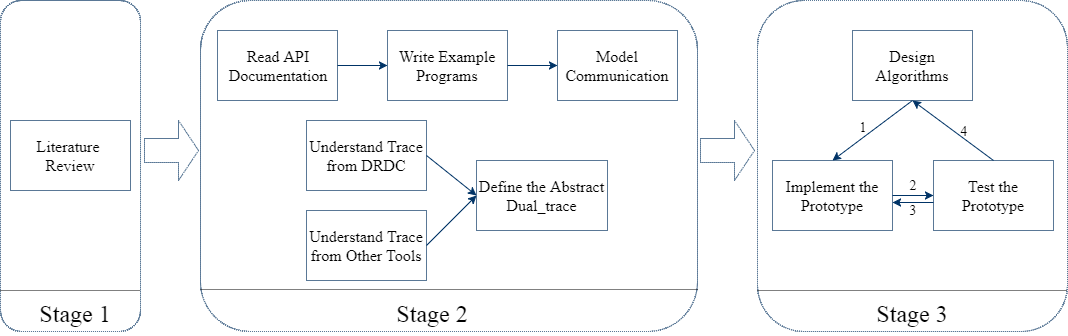
\includegraphics[scale=0.45]{Figures/methodology}}
  \caption{Research Approach overview}
  \label{methodology}
  \end{figure}

This research requires background knowledge of software security and vulnerabilities. I acquired the background knowledge basically from literature review. It helped me grab the essential concepts of software vulnerabilities and their categories, understand some facilities for vulnerabilities detection and software maintenance in the perspective of security. After that, I was convinced that communication analysis in assembly trace level would benefit software security engineers to understand the behaviour of software and detect software vulnerabilities. 

In order to analyze the communication of programs, I had to know how the communication works. For this purpose, I started the investigation by writing example simple programs with the Windows API and run them locally in my desktop. By understanding their behaviour and reading the Windows API documentation, I abstracted the communication model which is not operating system specific.

The abstract assembly trace definition was build on the generalization of the trace format provided by our research partner, DRDC. I don't have the access to their home-made assembly tracer which is based on PIN\cite{_pin_????}. Fortunately, they provideed me with a comprehensive document about the format of the captured trace and example traces. With these, I grasped the constructive view of the assembly execution trace. Further more, some other tools can also capture the required information in assembly level for communication analysis. This supports the generalization of the trace definition and the abstraction of the dual\_trace.

The implementation of the prototype and the communication analysis algorithms were developed in parallel. The high level communication identification algorithm and the specific algorithms for named pipe communication methods were abstracted based on the implementation, while the others are developed theoretically. Two experiments are designed to test this analysis method, the prototype and some algorithms. 


\section{Contributions}
The main contributions of these work can be summarized as:
\begin{itemize}
  \item \textbf{Communication Model:} The communication model in this thesis is an abstract model of the communications between two programs. It was abstracted from the understanding of several communication methods and is general for other communication methods that are not mentioned in this thesis.
  \item \textbf{Dual\_trace Formalization:} By understanding the assembly level execution traces, a dual\_trace was formalized to describe the information that needed for communication analysis. This model doesn't specify the format of the execution traces but defines what information is necessary to be contained to fulfil the analysis requirement. All execution traces that comply with this definition can be used for the analysis.
  \item \textbf{Communication Analysis Approach:} The overall approach to identify the communications in the dual\_trace is designed. Some algorithms were developed for the steps in this
approach regarding some communication methods or communication types.
  \item \textbf{Prototype:} A prototype is designed and implemented on Atlantis. This prototype demonstrate that the communication analysis approach is feasible. It is a unique tool for the security engineers to analyze the communications of programs via assembly execution trace analysis.
\end{itemize}

\section{Thesis Organization}
In Chapter 2, I summarize the related background information and knowledge needed to understand or related to this work including security and vulnerability, program communication mechanisms, program execution trace tools, and Atlantis. 

Chapter 3 describes the model of the communication between two programs. This model defines the communication in the context of trace analysis and discusses the properties of the communications. 

In Chapter 4, I first present the abstract dual\_trace formulation. Based on this formulation, I describe the communication analysis process and the essential algorithms.

In chapter 5, I present the implementation of a dual\_trace communication analysis prototype. 

In chapter 6, I present two experiments of communication analysis with dual\_traces using the implemented prototype. Notably, the result shows the communications are correctly identified. 

Finally, In chapter 7, I conclude the result of this research and outline the possible future work.
	%\startchapter{Methodology}
The Methodology used for this work composed of 7 major steps. To make this work executable, 1)I defined the problem by understanding the requirement from our research partner DRDC. 2) I obtained the related background knowledge by literature review. Then 3) I model the abstract communication channels. Based on these channel models,4) I develop algorithms to synchronize the communication events happen in the channel. After that, 5) I match the real channels used in Windows Communication Foundation to my channel models, verify their consistency with my models. Finally 6)I implement the synchronization algorithms for the dual-trace analysis and verify them by the dual-traces from DRDC.


\label{chapter:problem}

\newlength{\savedunitlength}
\setlength{\unitlength}{2em}
\section{Define the Problem}
A dual-trace consists of two execution traces that are generated from two interacting applications. The trace analysis is based only on the assembly level execution trace which contain the instructions and memory change of a running application. Beside all the factors in single trace analysis, dual-trace analysis has to analyze the communications of the applications in the traces. A communication between two applications including the communication channel open, all data exchanging events, the communication channel close.  Correspondingly, a full communication definition in the dual-trace should consist of the channel opening events in both sides, data sending and receiving events, and the the channel closing events in both sides. Each of these events consist of function call and related data from the memory record. In some cases there might be some events lacking from the trace, such as no data exchange after a channel is open, or the traces end before the channel was closed. However, the channel open is critical, without that there is no way to locate all other events in the traces. The goal communication analysis of dual-trace is to rebuild all the user concerned communication channels from the dual-trace.


\section{Obtain Background Knowledge}
I did a some background reading in the reverse engineering filed, focusing more on the vulnerabilities detection domain to better understand the current state and needs. In addition, to locate the communication event of the dual-trace, I need to investigate the communication methods' APIs to understand their structure in the assembly level traces. I need to know how the functions for channel setup and the functions for messages sending/receiving work. The system functions I was looking for is in C++ level. I have to know the C++ function names, related parameters, return value and so on. Furthermore, to understand their structure in the assembly level trace, I have to know the calling conventions in assembly, such registers/memory for parameters or return value.

\section{Model the Communication Channels}
There are two abstract models for communication based on the communication behavior. One is the order guaranteed communication model and the other is order in-guaranteed communication model. I define  how the communication happens as well as all the data send/receive scenario in each model. Later on the real communication channels will be categorized into these two models. 


\section{Develop the Dual Trace Synchronization Algorithms}


\section{Apply the Channel Models to Windows APIs}
I investigate 4 types of communication channels in Windows Communication Foundation and match each of them to the developed channel model. These 4 types are Only Named pipe, MQMS, HTTP, and TCP/UDP socket. The matching includes two steps: 1. Put each type of communication channel in the modeling categories by verify the existence of the message send/receive scenario. 2. Define the function callings for each event types in the channel, such as channel opening and closing, data sending and receiving. 

\section{Implement the Trace Synchronization Algorithms}

\section{Evaluate the Communication Channel Rebuilt Feature in Atlantis}



\setlength{\unitlength}{\savedunitlength}

	\startchapter{Background}
\label{chapter:Bac}
In this section, I summarize the background knowledge or information that related to this work. First I generally describe software vulnerability. Second, I discuss the general definition of communication among programs and their categorization. Third, I introduce some tools for assembly level program debugging and analysis. Finally I introduce Atlantis, the existing assembly level execution trace analysis environment, on which the implementation of this work based.

\section{Software Vulnerability}
Software vulnerability detection is one of the use cases of the communication analysis with assembly level execution traces. The understanding of fundamentals of software vulnerability is necessary to comprehend some implicit concepts or design intention through out this thesis. 

Vulnerabilities, from the point of view of software security, are specific flaws or oversights in a program that can be exploited by attackers to do something maliciousexpose such as modify sensitive information, disrupt or destroy a system, or take control of a computer system or program. They are considered to be a subset of bugs. Input and Data Flow, interface and exceptional condition handling where vulnerabilities are most likely to surface in software and memory corruption is one of the most common vulnerabilities. The awareness of these two facts would make the security auditing and vulnerabilities detection have more clear focus. \cite{dowd_art_2006}

\section{Program Communications}
Programs can communicate with each other via diverse mechanisms. The communication happens among processes is known as inter-process communication. This refers to the mechanisms an operating system provides the process to share data with each other. It includes methods such as signal, socket, message queue, shared memory and so on.\cite{garrido2000inter} This communications can happen over network or inside a device. Based on their reliability, the communication methods can be simply divided into two categories: reliable communication and unreliable communication. In this work, communication methods belong to all both categories has been covered. However, I only discuss the message based communication methods while leave the control based communication, like remote function call for the future.

\section{Program Execution Tracing in Assembly Level}
The communication analysis discuss throughout this thesis is based on the assembly traces. Thurs capturing of the execution traces became a prerequisite of this work. DRDC has its own home-made tracer, the traces from which are used in the experiments of this research. However, the model and algorithms developed in this research is not limited with this specific home-made tracer. Any tracer that can capture sufficient information according to the model can serve this purpose.

There are many tools that can trace a running program in assembly instruction level.  IDA pro \cite{eagle_ida_2008} is a widely used tool in reverse engineering which can capture and analysis system level execution trace. Giving open plugin APIs, IDA pro allows plugin such as Codemap \cite{_c0demap/codemap:_????} to provide more sufficient features for "run-trace" visualization. PIN\cite{_pin_????} as a tool for instrumentation of programs, provides a rich API which allows users to implement their own tool for instruction trace and memory reference trace. Other tools like Dynamic \cite{brueningqz} and OllyDbg\cite{yuschuk2007ollydbg} also provide the debugging and tracing functionality in assembly level. 

\section{Atlantis}
Atlantis is a trace analysis environment developed in Chisel. It can support analysis for multi-gigabyte assembly traces. There are several features distinct it from all other existing tools and make it particularly successful in large scale trace analysis. These features are 1) reconstruction and navigation the memory state of a program at any point in a trace; b) reconstruction and navigation of system functions and processes; and c) a powerful search facility to query and navigate traces. The work of this thesis is not a extension of Atlantis. But it take advantages of Atlantis by reusing it existing functionality to assist the dual\_trace analysis.





    \externaldocument{../appendix/chapter_app}
\startchapter{Modeling}
\label{chapter:Mod}
In this chapter, I modeled the communication of two running programs. The modeling are based on the investigation of some common used communication methods. The communication methods are divided into two categories based on their data transmission properties. The terminology of using in this chapter can be found in \ref{term}.

\section{Communication Categorization and Communication Methods}
In general, there are two types of communication: reliable and unreliable in the terms of their reliability of data transmission. The reason to divide the communication methods into these two categories is that the data transmission properties of the communications fall in different categories affect the mechanism of the data verification in the identification algorithm. In the following two subsections, I summarize the characteristics of these two communication categories. The communication methods list in Table\ref{methodsInCategories} will be discussed further to provide more concrete comprehension. 
\begin{table}[H]
\centering
\caption{Communication Methods Discussed in This Work}
\label{methodsInCategories}
\begin{tabular}{|l|l|}
 \hline
\textbf{Reliable Communication}& \textbf{Unreliable Communication}\\
 \hline
Named Pipes & Message Queue   \\
TCP &  UDP \\
 \hline
\end{tabular}
\end{table}


\subsection{Reliable Communication}\label{reliable}
A reliable communication guarantees the data being sent by one endpoint of the channel is always received losslessly and in the same order in the other endpoint. For some communication methods, a channel can be closed before all sent data being received. With this property, the concatenated data in the receive stream of one endpoint should be the prefix of the concatenated data in the send stream of the other endpoint(potentially equal). Therefore, comparing the concatenated received data of one endpoint to the concatenated sent data of the other can verify the send and receive data.

\subsection{Unreliable Communication}\label{unreliable}
An unreliable communication does not guarantee the data being sent always arrive the receiver. Moreover, the data packets can arrive to the receiver in any order. However, the bright side of unreliable communication is that the packets being sent are always arrived as the origin packet, no data re-segmentation would happen. Accordingly, the send and receive data verification can be done by matching the data packet in a receive event to the data packet in a send event on the other side.

\subsection{Communication Methods}
In this section, I describe the mechanism and the basic data transfer characteristics of each communication method in Table\ref{methodsInCategories} briefly. Moreover, data transfer scenarios are represented correspondingly in diagrams for each communication method. 
 
\subsubsection{Named Pipe}
A named pipe provides FIFO communication mechanism for inter-process communication. It can be a one-way or a duplex pipe. \cite{khambattinamed}

The basic data transfer characteristics of Named Pipe are:
\begin{itemize}
  \item Bytes are received in order
  \item Bytes sent as a segment can be received in multiple segments(the opposite is not true)
  \item No data duplication
  \item If a sent segment is loss, all the following segments will lost(this happen when the receiver disconnect from the channel) 
  
\end{itemize}

Based on these characteristics, the data transfer scenarios of Named pipe can be exemplified in Figure\ref{namedpipe}. 
\begin{figure}[H]
\centerline{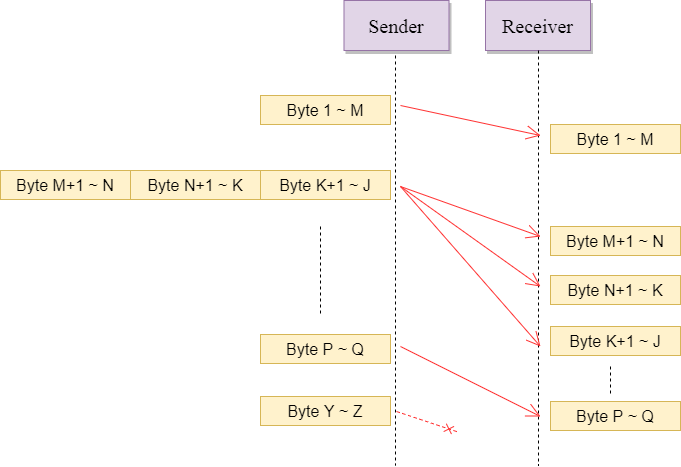
\includegraphics[scale=0.48]{Figures/namedpipe}}
\caption{Data Transfer Scenarios for Named Pipe}
\label{namedpipe}
\end{figure}

\subsubsection{Message Queue}
Message Queuing (MSMQ) is a communication method to allow applications which are running at different times across heterogeneous networks and systems that may be temporarily offline can still communicate with each other. Messages are sent to and read from queues by applications. Multiple sending applications can send messages to and multiple receiving applications can read messages from one queue.\cite{redkar2004pro} In this work, only one sending application versus one receiving application case is considered. Multiple senders to multiple receivers scenario can be divided into multiple sender and receiver situation. Both applications of a communication can send to and receive from the channel.

The basic data transfer characteristics of Message Queue are:
\begin{itemize}
  \item Bytes sent in packet and received in packet, no bytes re-segmented
  \item Packets can lost
  \item Packets received in order
  \item No data duplication
\end{itemize}
Based on these characteristics, the data transfer scenarios of Message Queue can be exemplified in Figure\ref{msmq}.
\begin{figure}[H]
\centerline{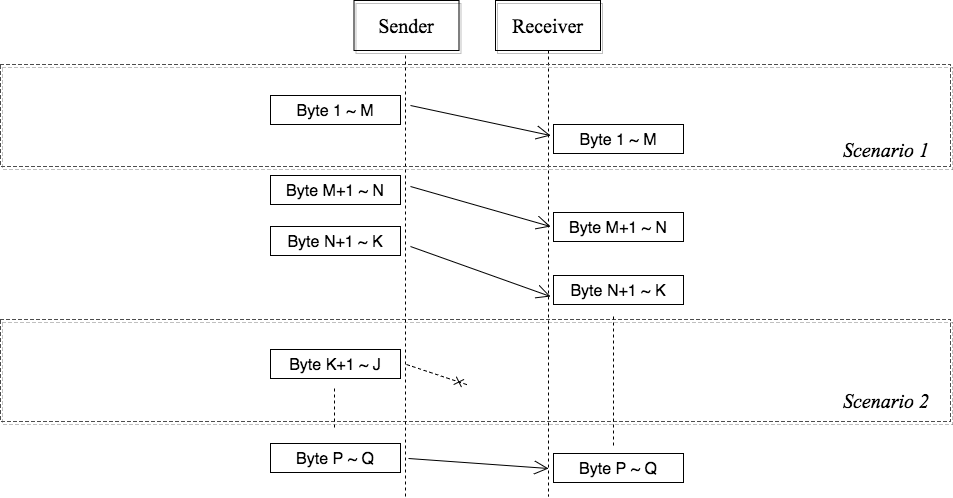
\includegraphics[scale=0.48]{Figures/msmq}}
\caption{Data Transfer Scenarios for Message Queue}
\label{msmq}
\end{figure}

\subsubsection{TCP}
TCP is the most fundamental reliable transport method in computer networking. TCP provides reliable, ordered, and error-checked delivery of a stream of octets between applications running on hosts in an IP network. The TCP header contains the sequence number of the sending octets and the acknowledge sequence this endpoint is expecting from the other endpoint(if ACK is set). The re-transmission mechanism is based on the ACK. 

The basic data transfer characteristics of TCP are:
\begin{itemize}
  \item Bytes received in order
  \item No data lost(lost data will be re-transmitted)
  \item No data duplication
  \item Sender window size is different from receiver's window size, so packets can be re-segmented
\end{itemize}

Based on these characteristics,  the data transfer scenarios of TCP can be exemplified in Figure\ref{tcp}.
\begin{figure}[H]
\centerline{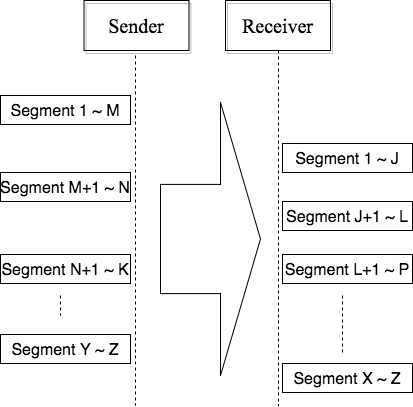
\includegraphics[scale=0.48]{Figures/tcp}}
 \caption{Data Transfer Scenarios for TCP}
\label{tcp}
\end{figure}

\subsubsection{UDP}
UDP is a widely used unreliable transmission method in computer networking. It is a simple protocol mechanism, which has no guarantee of delivery, ordering, or duplicate protection. This transmission method is suitable for many real time systems. 

The basic data transfer characteristics of UDP are:
\begin{itemize}
  \item Bytes sent in packet and received in packet, no re-segmentation
  \item Packets can lost
  \item Packets can be duplicated
  \item Packets can arrive receiver out of order
\end{itemize}

Based on these characteristics, the data transfer scenarios of UDP can be exemplified in Figure\ref{upd}.
\begin{figure}[H]
\centerline{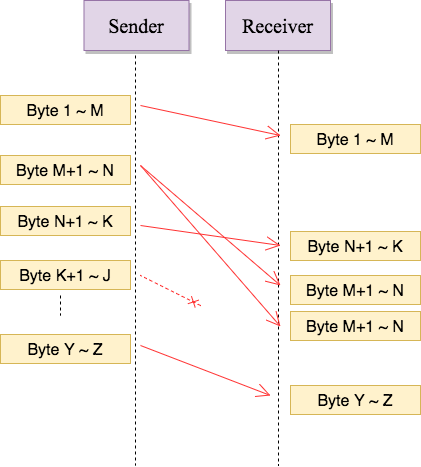
\includegraphics[scale=0.48]{Figures/udp}}
 \caption{Data Transfer Scenarios for UDP}
\label{upd}
\end{figure}

\section{Communication Model}\label{definition}
The communication of two programs is defined in this section. The communication in this work is data transfer activities between two running programs through a specific channel. Some collaborative activities between the programs such as remote procedure call is out of the scope of this research. Communication among multiple programs (more than two) is not discussed in this work. The channel can be reopened again to start new communications after being closed. However, the reopened channel will be treated as a new communication. The way that I define the communication is leading to the communication identification in the dual-trace. So the definition is not about how the communication works but what it looks like. There are many communication methods in the real world and they are compatible to this communication definition. 

\subsection{Communication Definition}
In the context of a dual\_trace, a communication is a sequence of data transmitted between two endpoints through a communication channel. The endpoints connect to each other using the identifier of this channel. We therefore defined a communication c as a triplet:

$c =<ch, e_0, e_1>$

where $e0$ and $e1$ are endpoints while $ch$ is the communication channel used (e.g. a named piped located at /tmp/pipe).

From the point of view of traces, the endpoints $e_0$ and $e_1$ are defined in terms of three properties: the handle created within a process for the endpoint for subsequent operations(e.g. data send and receive), the data stream received and the data stream sent. Therefore, I define an endpoint e as a triplet:

$ e =<handle, d_r, d_s>$

where $d_r$ and $d_s$ are data streams. A data stream is a sequence of events, each sends or receives a package. Each package contains data that is being sent or received (its payload). Hence, we can define a data stream $d$ as a sequence of $n$ packages:

$ d = (pk_1, pk_2, ..., pk_n)$ 

Note that this is the sequence of packages as seen from the endpoint and might be different than the sequence of packages seen in the other endpoint, specially where there is package reordering, loss or duplication.

Each package has several attributes:
\begin{itemize}
\item \textit{Relative time(it was sent or received):} In a trace, we do not have absolute time for an event. However, we know when when an event (i.e. sending or receiving a package) has happened with respect to another event. we will use the notation 

$time(pkg)$ 

to denote this relative time. Hence, if  $i < j $ , then 

$time(pk_i) < time(pk_j)$

\item \textit{Payload:} Each package has a payload (the data being sent). This payload can be modeled as a string contained in the package.we will use the notation 

$pl(pkg)$ 

to denote this payload. 

\end{itemize}


\subsection{Communication Properties}
The properties of the communications can be described based on the definition of the communication.

\subsubsection{Properties of reliable communication:}
A reliable communication guarantees that the data sent and received between a package happens without loss and in the same order.

For a given data stream, I will define the data in this stream as the concatenation of all the payloads of all the packages in this stream, in the same order, and denote is as $data(d)$.

Given $ d = <pk_1, pk_2, ..., pk_n>$, $data(d) = pl(pk_1) \cdot pl(pk_2)\cdot \ldots \cdot pl(pk_n)$


\begin{itemize}
 \item \textit{ Content Preservation:} for a communication:

$c = <ch, <h_0, dr_0, ds_0>, <h_1, dr_1, ds_1>>$

the received data should always be a prefix (potentially equal) of the data sent:

$data(dr_0)$ is a prefix of $data(ds_1)$  and

$data(dr_1)$ is a prefix of $data(ds_0)$

 \item \textit{Timing Preservation:} at any given point in time, the data received by an endpoint should be a prefix of the data that has been sent from the other:
 
for a sent data stream of size $m$, $ds= <pks_1, pks_2, ... pks_m>$ that is received in data stream of size $n$, $dr = <pkr_1, pkr_2, ... pkr_n>$

for any $k \in {1..n}$, there must exist $j \in {1..m}$ such that: $pks_j$ was sent before $pkr_k$ was received:

$  time(pks_j) < time(pkr_k)$

  and

$  data(<pkr_1, pkr_2, ..., pkr_k>)$ is a prefix of $data(<pks_1, pks_2, ..., pks_j>)$

  In other words, at any given time, the recipient can only receive at most the data that has been sent.

\end{itemize}

\subsubsection{Properties of unreliable communication:}
In unreliable communication sender and receiver are not concerned with the concatenation of packages. Instead, they treat each package independent of each other.
\begin{itemize}
 \item \textit{ Content Preservation:} a package that is received should have been sent:

for a sent data stream of size $m$, $ds= <pks_1, pks_2, ... pks_m>$ that is received in data stream of size $n$, $dr = <pkr_1, pkr_2, ... pkr_n>$

for any $pkr_j \in dr$ there must exist $pks_i \in ds$

We will say that the $pkr_j$ is the matched package of $pks_i$, and vice-versa, $pks_i$ is the matched package of $pkr_j$, hence

$match(pkr_j) = pks_i$  and

$match(pks_i) = pkr_j$

 \item \textit{Timing Preservation:}  at any given point in time, packages can only be received if they have been sent

  for a sent data stream of size $m$, $ds= <pks_1, pks_2, ... pks_m>$ that is received in data stream of size $n$, $dr = <pkr_1, pkr_2, ... pkr_n>$

  for any $k \in {1..n}$, $time(match(pkr_j)) < time(pkr_j)$

In other words, the match of the received package must has been sent before it is received.

\end{itemize}



In the following two examples, $h_0$ and $h_1$ are the handles of the two endpoints $e_0$ and $e_1$ of the communications. $ds_0$, $dr_0$ and $ds_1$, $dr_1$ data streams of the endpoints $e_0$ and $e_1$. The string payloads are the strings represented in blue and red in the figures. 

Figure\ref{reliableexample} is an example of the reliable communication. 

\begin{figure}[H]
\centerline{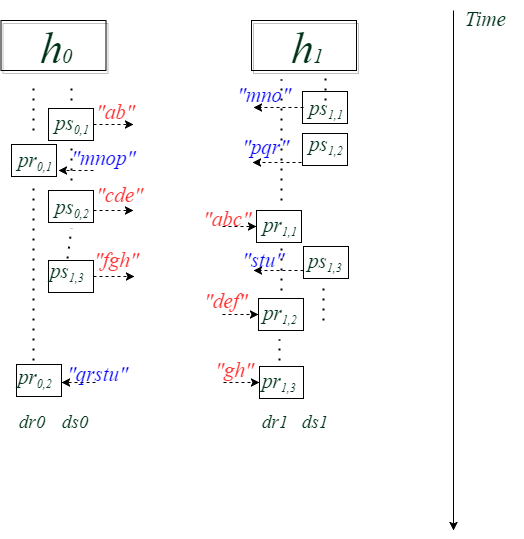
\includegraphics[scale=0.55]{Figures/reliableexample}}
\caption{Example of Reliable Communication}
\label{reliableexample}
\end{figure}

In this example, the payloads of the packages are:

$pl(pks_01)=``ab"$, $ pl(pks_02)=``cde"$, $pl(pks_03)=``fgh"$;

$pl(pkr_11)=``abc"$, $pl(pkr_12)=``def"$, $pl(pkr_13)=``gh"$ .

and 

$pl(pks_11)=``mno"$, $pl(pks_12)=``pqr"$, $pl(pks_13)=``stu"$;

$pl(pkr_01)=``mnop"$, $pl(pkr_02)=``qrstu"$. 

on the other direction. Their properties:

$pl(pks_01) \cdot pl(pks_02) \cdot pl(pks_03) = pl(pkr_11) \cdot pl(pkr_12) \cdot pl(pkr_13) = ``abcdefgh"$ and 

$pl(pks_11) \cdot pl(pks_12) \cdot pl(pks_13) = pl(pkr_01) \cdot pl(pkr_02) = ``mnopqrstu"$. 

satisfy the content preservation. 

The relative time relationship of the packages are: 

$time(pks_01) < time(pks_02) < time(pkr_11)< time(pks_03) < time(pkr_12) < time(pkr_13) $;

$time(pks_11) < time(pks_12) < time(pkr_01)< time(pks_13) < time(pkr_02)$. 

The fact that
 
$pl(pkr_01) = ``mnop"$ is the prefix of $pl(pks_11) \cdot  pl(pks_12) = ``mnopqr"$,

$pl(pkr_01) \cdot pl(pkr_02)=``mnopqrstu"$ is the prefix of(is this case identical to ) $pl(pks_11) \cdot pl(pks_12) \cdot pl(pks_13) = ``mnopqrstu" $,  

$pl(pkr_11)=``abc"$ is the prefix of $pl(pks_01 \cdot pl(pks_02) = "abcde"$,  

$pl(pkr_11) \cdot pl(pkr_12)= ``abcdef"$ and  $pl(pkr_11) \cdot pl(pkr_12) \cdot pl(pkr_13) = ``abcdefgh"$ are  the prefix of  $pl(pks_01) \cdot pl(pks_02) \cdot pl(pks_03)= ``abcdefgh"$

satisfy the timing preservation. 


Figure\ref{unreliableexample} is an example of the unreliable communication. 

\begin{figure}[H]
\centerline{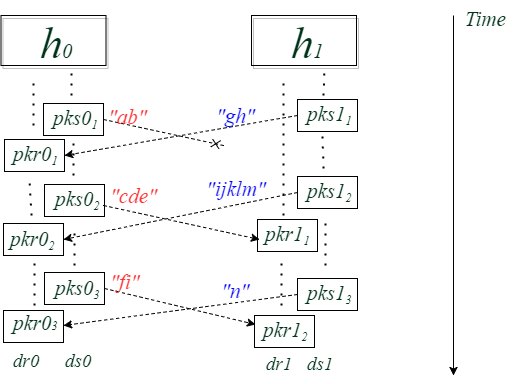
\includegraphics[scale=0.55]{Figures/unreliableexample}}
\caption{Example of Unreliable Communication}
\label{unreliableexample}
\end{figure}

In this example:

$pkr_11 = pks_02=``cde"$, $time(pkr_11) > time(pks_02)$; 

$pkr_12 = pks_02=``cde"$, $time(pkr_12) > time(pks_02)$; 

$pkr_13 = pks_03=``fi"$, $time(pkr_13) > time(pks_03)$;

$pkr_01 = pks_11=``gh"$, $time(pkr_01) > time(pks_11)$;

$pkr_02 = pks_12=``ijklm"$, $time(pkr_02) > time(pks_12)$;

$pkr_03 = pks_13=``n"$, $time(pkr_03) > time(pks_13)$.

All of these satisfy the content preservation and timing preservation of the unreliable communication.


    %\startchapter{Apply the Model on Windows C++ API}
\label{chapter:Mod}
In this section, I investigated 4 different channel types: Named pipes, MQMS, TCP/UDP socket and HTTP channels, all of which are the most fundamental ones in Windows communication framework. By matching these channels to the communication model I verified generality of the modeling. 


\section{Named Pipes Channel}
A named pipe is a named, one-way or duplex pipe for communication between the pipe server and one or more pipe clients. Both the server and client can read or write into the pipe. The pipe server and client can be on the same or different computers.  In here we only consider one server V.S one client dual-trace. One server to multiple clients scenario can always be divided into multiple server/client dual-traces. We call the end of the named pipe instance. An instance can be a server instance or a client instance. All instances of a named pipe share the same pipe name, but each instance has its own buffers and handles, and provides a separate conduit for client/server communication. 

A named pipe server responsible for the creation of the pipe, while clients of the pipe can connect to the server after it created. The creation and connection of a named pipe will return the handle ID of that pipe. As we mention before, each instance has its own handles, so the returned handle IDs of the pipe creation function of the server and pipe connection function from each client are different. These handler IDs will be used later on when messages are being sent or received to specify a pipe to which send.

\subsection{Important Channel Parameters}
There are many options for a named pipe. Some of them are critical in the perspective of the channel operations. In this sections we list the important ones.

\subsubsection{Blocking/Non-Blocking}
The named pipe channel can be opened in blocking mode or non-blocking mode. In blocking mode, when the pipe handle is specified in the ReadFile, WriteFile, or ConnectNamedPipe function, the operations are not completed until there is data to read, all data is written, or a client is connected. In non-blocking mode, ReadFile, WriteFile, and ConnectNamedPipe always return immediately. The operation fail if the channel is not ready for read, write or connection. However, since in this work we only aimed at locating the successful communication, as long as the operations success, we can locate them no matter the pipe is in blocking or non-blocking mode.

\subsubsection{Synchronous/Asynchronous}
Another critical option for named pipe channel is Synchronous/Asynchronous. In Synchronous mode, the ReadFile, WriteFile TracnsactNamedPipe and connectNamedPipe functions does not return until the operation it is performing is completed. That means we can retrieve the sent/receive message in the trace when the function return. When the channel is enable overlapped mode, the ReadFile, WriteFile TracnsactNamedPipe and connectNamedPipe functions perform asynchronously. In the asynchronous mode, ReadFile, WriteFile, TransactNamedPipe, and ConnectNamedPipe operations return immediately regardless if the operations are completed. And if the function call return ERROR\_IO\_PENDING, the calling thread then call the GetOverlappedResult function to determine the results. For the read operation, the message will be stored in the buffer indicated in the ReadFile function call when the read operation complete successfully.

\subsection{Send/Receive Scenarios}
In section \ref{modmatchresult}, I defined 13 scenarios of the general communication channel. In this section, I check their existence for named pipe channel. Some important properties of named pipe channel, which affecting the happening of the scenarios are listed in Table \ref{namedpipeproperties}. The result of the existence of the scenarios is list in Table\ref{pipematchresult} with the explanation by the affecting properties. 

\begin{table}[h]
\centering
\caption{Named Pipe Channel properties}
\label{namedpipeproperties}
\begin{tabular}{|l|p{12cm}|}
\hline
\begin{tabular}[c]{@{}l@{}}\textbf{Property} \end{tabular} & \begin{tabular}[c]{@{}l@{}}\textbf{Description}\end{tabular}\\ \hline
1 & All message going into the pipe will go out in order      \\ \hline
2 & The receiver can read multiple times to get the whole message, when he send message size is larger than the receiver's buffer  \\ \hline
3 & The receiver can only read contents from one write operation on the other end of the pipe in its one read operation                                            \\ \hline
4 & Read/Write operation return immediately when error occurs\\\hline
\end{tabular}
\end{table}

\begin{table}[h]
\centering
\caption{Send/Receive Scenarios of Named Pipe}
\label{pipematchresult}
\begin{tabular}{|l|l|l|}
\hline
\begin{tabular}[c]{@{}l@{}}\textbf{Scenario} \end{tabular} & \begin{tabular}[c]{@{}l@{}}\textbf{Existence}\end{tabular} & \begin{tabular}[c]{@{}l@{}}\textbf{Comment}\end{tabular}\\ \hline
Scenario 1 & YES & Property 1                       \\ \hline
Scenario 2 & NO  & Property 1 \\ \hline
Scenario 3 & YES & Property 4             \\ \hline
Scenario 4 & YES & Property 2 \\ \hline
Scenario 5 & NO  & Property 1                                         \\ \hline
Scenario 6 & NO  & Property 1 \\ \hline
Scenario 7 & NO  & Property 1 \\ \hline
Scenario 8 & NO  & Property 3         \\ \hline
Scenario 9 & NO  & Property 3                                                \\\hline
Scenario 10 & NO & Property 3                                               \\ \hline
Scenario 11 & NO & Property 3                                                 \\ \hline
Scenario 12 & NO & Property 3                                                 \\ \hline
Scenario 13 & NO & Property 3                                                 \\ \hline
\end{tabular}
\end{table}


\begin{figure}[h]
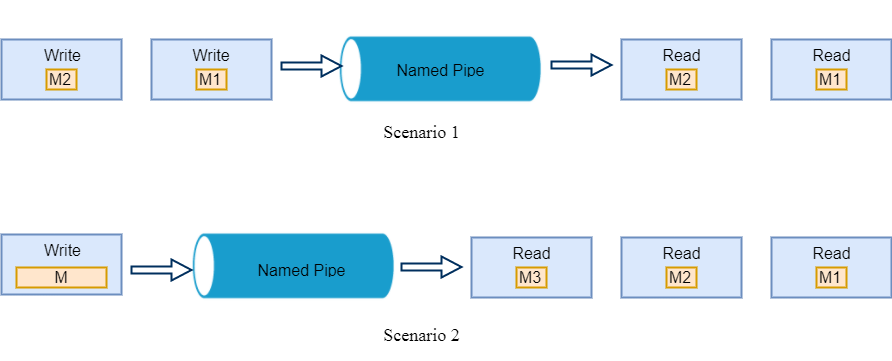
\includegraphics[scale=.48]{Figures/event}
 \caption{Two successful write/read operation scenarios. Each blue block indicate a single read or write operation.}
\label{event}
\end{figure}


\subsection{Function Calls In Each Communication Stage}
As we talk in the parameters section, Synchrounous and Asychronous mode affect the functions used to complete the send and receive operation as well as the operation of the functions. In the follow subsections, we will list the related functions for the named pipe channel for both synchronous mode and asynchronous mode. The create channel functions for both modes are the same but with different input parameters. The functions for send and receive message are also the same for both case. However, the operation of the send and receive functions are different for different mode. In addition, extra functions are being called to check the status of message sending or receiving in asynchronous mode.
\subsubsection{Synchronous}
We list all the functions that needed to locate an messaging event in a dual-trace in Table\ref{synfunctions} for synchronous named pipe. The Channel Open Functions indicate how the channel being opened/created in server and client sides, and they are different. The file name is an input parameter for CreateNamedPipe and CreateFile function. The client and server of the same pipe use the same file name. This is an important parameter to identify the pipe between the server and client in the traces. The File name is stored in the RCX register when the function is being called. The file handle is a integer return value from the CreateNamedPipe and CreateFile functions call. It will be stored in RAX register when the function return. This handle will be used as the identifier of a pipe in the client or server later on. The handle is different for server and each client even they connected to the same pipe. The send or receive message functions are the same in server and client. the file handle generated when the channel created are stored in register RCX when the WriteFile and ReadFile functions are being called. RDX holds the address of the buffer for message send or receive. The actual size of the message being sent or received are store in R9 when the function return.
  
    \begin{table}[h]
        \centering
        \caption{Functions for communication stages definition of synchronous named pipe}
        \label{synfunctions}
        \begin{tabular}{|p{1.8cm}|l|l|l|l|}
            \hline
             \multirow{2}{*}{\textbf{Stage}} &
               \multicolumn{2}{c|}{\textbf{Server}} &
               \multicolumn{2}{c|}{\textbf{Client}} \\
             \cline{2-5}
              & \textbf{Function}& \textbf{Parameters} & \textbf{Function} & \textbf{Parameters}  \\
             \hline
             \multirow{2}{*}{\parbox{1.8cm}{\textbf{Channel Open}}}
             &\multirow{2}{*}{\parbox{2.5cm}{CreateNamed- Pipe}} &  RAX: File Handler & \multirow{2}{*}{CreateFile} &  RAX: File Handler\\
              \cline{3-3} \cline{5-5}
             &&  RCX: File Name &  &  RCX: File Name\\
            \hline
             \multirow{6}{*}{\parbox{1.8cm}{\textbf{Message Send/Receive}}}
             &\multirow{3}{*}{WriteFile} &  RCX: File Handle & \multirow{3}{*}{WriteFile} &  RCX: File Handle\\
              \cline{3-3} \cline{5-5}
             &&  RDX: Buffer Address &  &  RDX: Buffer Address\\
                           \cline{3-3} \cline{5-5}
             & &  R9: Message Length &  &  R9: Message Length\\
            \cline{2-5}
             & \multirow{3}{*}{ReadFile}&  RCX: File Handle & \multirow{3}{*}{ReadFile} &  RCX: File Handle\\
              \cline{3-3} \cline{5-5}
              &&  RDX: Buffer Address &  &  RDX: Buffer Address\\
                           \cline{3-3} \cline{5-5}
             & &  R9: Message Length &  &  R9: Message Length\\
            \hline
           \multirow{2}{*}{\parbox{1.8cm}{\textbf{Channel Close}}}
             &\multirow{2}{*}{CloseHandle} & \multirow{2}{*}{RCX: File Handler} & \multirow{2}{*}{CloseHandle} &  \multirow{2}{*}{RCX: File Handler}\\
             &&   &  & \\
            \hline
        \end{tabular}
    \end{table}
\subsubsection{Asynchronous}
The functions used in Asynchronous mode for create channel, send and receive message are the same as those used in synchronous mode. However,  the ReadFile and WriteFile functions run asynchronously when the channel is asynchronous. This means the function will return immediately, even if the operation has not been completed. If the operation is complete when the function returns, the return value indicates the success or failure of the operation. Otherwise the functions return zero and GetLastError returns ERROR\_IO\_PENDING. In this case, the calling thread must wait until the operation has finished. The calling thread must then call the GetOverlappedResult function to determine the results. This means besides looking for ReadFile and WriteFile function calls in the traces, the GetOverlappedResult function should be checked in the traces to get the full result of the ReadFile or WriteFile operations. There are two scenarios of the successful communication in the dual-trace for asynchronous mode. The first one is exactly the same as synchronous situation. The second one involves the functions listed in Table\ref{asynfunctions}. In the later one, Read operation searching is bit more complicated, since ReadFile function has to be located first to get the buffer address, and then GetOverlappedResult function return should be search for the message retrieval from the memory.
    \begin{table}[h]
        \centering
        \caption{Functions for additional communication type definition of asynchronous named pipe}
        \label{asynfunctions}
        \begin{tabular}{|p{1.8cm}|l|l|l|l|}
            \hline
             \multirow{2}{*}{\textbf{Stage}} &
               \multicolumn{2}{c|}{\textbf{Server}} &
               \multicolumn{2}{c|}{\textbf{Client}} \\
             \cline{2-5}
              & \textbf{Function}& \textbf{Parameters} & \textbf{Function} & \textbf{Parameters}  \\
             \hline
             \multirow{2}{*}{\parbox{1.8cm}{\textbf{Channel Open}}}
             &\multirow{2}{*}{\parbox{2.5cm}{CreateNamed- Pipe}} &  RAX: File Handler & \multirow{2}{*}{CreateFile} &  RAX: File Handle\\
              \cline{3-3} \cline{5-5}
             &&  RCX: File Name &  &  RCX: File Name\\
            \hline
             \multirow{8}{*}{\parbox{1.8cm}{\textbf{Message Send/Receive}}}
             &\multirow{3}{*}{WriteFile} &  RCX: File Handle & \multirow{3}{*}{WriteFile} &  RCX: File Handle\\
              \cline{3-3} \cline{5-5}
             &&  RDX: Buffer Address &  &  RDX: Buffer Address\\
                           \cline{3-3} \cline{5-5}
             & &  R9: Message Length &  &  R9: Message Length\\
            \cline{2-5} 

             & \multirow{3}{*}{ReadFile}&  RAX: File Handle & \multirow{3}{*}{ReadFile} &  RCX: File Handle\\
              \cline{3-3} \cline{5-5}
              &&  RDX: Buffer Address &  &  RDX: Buffer Address\\
                           \cline{3-3} \cline{5-5}
             & &  R9: Message Length &  &  R9: Message Length\\
              \cline{2-5} 
             & \multirow{2}{*}{\parbox{2.5cm}{GetOver- lappedResult}}&  RCX: File Handler & \multirow{2}{*}{\parbox{2.5cm}{GetOver- lappedResult}} &  RCX: File Handler\\
              \cline{3-3} \cline{5-5}
             & &  RDX:  OVERLAPPED&  &  RDX:  OVERLAPPED\\
                         \hline
                         
                          \multirow{2}{*}{\parbox{1.8cm}{\textbf{Channel Close}}}
             &\multirow{2}{*}{CloseHandle} & \multirow{2}{*}{RCX: File Handler} & \multirow{2}{*}{CloseHandle} &  \multirow{2}{*}{RCX: File Handler}\\
             &&   &  & \\
            \hline
        \end{tabular}
    \end{table}
    


\section{MQMS Channel}
Message Queuing (MSMQ) is designed for communication between applications which is running at different times across heterogeneous networks and systems that may be temporarily offline. Messages are sent to and read from queues by applications. Multiple sending applications can send messages to and multiple receiving applications can read messages from one queue. \cite{redkar2004pro}

However, in this work only one sending application versus one receiving application case is considered. Multiple sender to multiple receiver scenario can always be divided into multiple sender/receiver dual-traces. 

The sending or receiving application can create the queue or use the existing one. However, both of them have to open the queue before they access it. The handle ID returned by the open queue function will be used later on when messages are being sent or received

\subsection{Important Channel Parameters}    
Same as Named pipe channels, MSMQ channel have many options or settings affecting the operations happen in the channels. In this section I listed those ones affecting the dual trace analysis. 

\subsubsection{Synchronous/Asynchronous Receiving}
In Message Queuing channels, only receiving can operate in asynchronous mode. When synchronously reading messages, the input parameters fnReceiveCallback and lpOverlapped are set to NULL. The calling thread is blocked until a suitable message is available or a time-out occurs for the receiving function. When asynchronously reading messages, MQReceiveMessage returns MQ\_OK if a suitable message is found. Otherwise, MQReceiveMessage returns immediately with the return value MQ\_INFORMATION\_OPERATION\_PENDING. This return value indicates that the operation is pending and will be completed as soon as a suitable message can be found. Further operations needed to get the message later on. More details about the further operations will be described in Section \ref{callback}
\subsubsection{Asynchronous Receiving With Call Back Functio or Completion port}\label{callback}
When the receiving operates in asynchronous mode, completion ports or call back function can be used for the asynchronously reading. 

In the completion port using situation, MQGetOverlappedResult is called to retrieve the success or error code from the OVERLAPPED structure. If no message is received before the time-out period elapses, an error is returned, and the start routine returns, terminating the thread in an implicit call to ExitThread.

In the call back function using situation, a call back function's pointer is given when the receiving function is being called. The call back function will perform its task as long a message was received or the time-out interval supplied by the caller elapsed.
\subsubsection{Message Properties Description Structure}

\subsection{Send/Receive Scenarios}
In this section, I check the scenarios existence for message queuing. Some important properties of MSMQ channel, which affecting the happening of the scenarios are listed in Table \ref{msmqproperties}. The result of the existence of the scenarios is list in Table\ref{msmqmatchresult} with the explanation by the affecting properties. 

\begin{table}[h]
\centering
\caption{Named Pipe Channel properties}
\label{msmqproperties}
\begin{tabular}{|l|p{12cm}|}
\hline
\begin{tabular}[c]{@{}l@{}}\textbf{Property} \end{tabular} & \begin{tabular}[c]{@{}l@{}}\textbf{Description}\end{tabular}\\ \hline
1 & All message going into the pipe will go out in order      \\ \hline
2 & The receiver can read multiple times to get the whole message, when he send message size is larger than the receiver's buffer  \\ \hline
3 & The receiver can only read contents from one write operation on the other end of the pipe in its one read operation                                            \\ \hline
4 & Read/Write operation return immediately when error occurs\\\hline
\end{tabular}
\end{table}

\begin{table}[h]
\centering
\caption{Send/Receive Scenarios of Named Pipe}
\label{msmqmatchresult}
\begin{tabular}{|l|l|l|}
\hline
\begin{tabular}[c]{@{}l@{}}\textbf{Scenario} \end{tabular} & \begin{tabular}[c]{@{}l@{}}\textbf{Existence}\end{tabular} & \begin{tabular}[c]{@{}l@{}}\textbf{Comment}\end{tabular}\\ \hline
Scenario 1 & YES & Property 1                       \\ \hline
Scenario 2 & NO  & Property 1 \\ \hline
Scenario 3 & YES & Property 4             \\ \hline
Scenario 4 & YES & Property 2 \\ \hline
Scenario 5 & NO  & Property 1                                         \\ \hline
Scenario 6 & NO  & Property 1 \\ \hline
Scenario 7 & NO  & Property 1 \\ \hline
Scenario 8 & NO  & Property 3         \\ \hline
Scenario 9 & NO  & Property 3                                                \\\hline
Scenario 10 & NO & Property 3                                               \\ \hline
Scenario 11 & NO & Property 3                                                 \\ \hline
Scenario 12 & NO & Property 3                                                 \\ \hline
Scenario 13 & NO & Property 3                                                 \\ \hline
\end{tabular}
\end{table}



\subsection{Function Calls In Each Communication Stage}
We list all the functions that needed to locate an messaging event in a dual-trace in Table\ref{synfunctions} for MSMQ. The Channel Open Functions indicate how the channel being opened in sending and receiving sides. The Queue Format Name is an input parameter for MQOpenQueue function. This is an important parameter to identify the queue. The File name is stored in the RCX register when the function is being called. The queue handle is a integer return value from the MQOpenQueue functions call. It will be stored in RAX register when the function return. The handle is different for each application using the same queue. The queue handle generated when the queue is opened by an application are stored in register RCX when the MQSendMessage or MQReceiveMessage functions are being called for message sending and receiving. RDX holds the address of the sending message structure for message sending while R9 holds the address of the receiving message structure for message receiving. For message receiving, the operation can be synchronous or asynchronous. For the asynchronous receiving, an callback function's pointer is indicated in the parameter fnReceiveCallback which is pushed on the stack if the callback function is employed. If the call back function is not employed, MQGetOverlappedResult should be called to get the received message.

\subsubsection{Synchronous Receiving}
The functions used for defining a communication channel and events are listed in Table\ref{msmqsynfunctions}.
    \begin{table}[h]
        \centering
        \caption{Functions for communication stages of MSMQ for synchronous receiving}
        \label{msmqsynfunctions}
        \begin{tabular}{|l|l|l|}
            \hline
             \textbf{Stage} & \textbf{Function}& \textbf{Parameters}  \\
             \hline
             \multirow{2}{*}{{\textbf{Channel Open}}}
             &\multirow{2}{*}{{MQOpenQueue}} &  RAX: Queue Handler\\
              \cline{3-3} 
             & &  RCX: Queue Format Name\\
            \hline
             \multirow{4}{*}{{\textbf{Message Send/Receive}}}
             &\multirow{2}{*}{MQSendMessage} &  RCX: Queue Handle \\
              \cline{3-3} 
             &&  RDX: Message description structure Address \\
            \cline{2-3}
             & \multirow{2}{*}{MQReceiveMessage}&  RCX: Queue Handle \\
              \cline{3-3} 
              &&  R9: Message description structure Address \\
            \hline
            \textbf{Channel Close} &MQCloseQueue & RCX: Queue Handler \\
            \hline
        \end{tabular}
    \end{table}

\subsubsection{Asynchronous Receiving with Call Back Functions}
The functions used for defining a communication channel and events are listed in Table\ref{msmqasynfunctionscallback}.
    \begin{table}[h]
        \centering
        \caption{Functions for communication stages of MSMQ for asynchronous receiving with call back function}
        \label{msmqasynfunctionscallback}
        \begin{tabular}{|l|l|l|}
            \hline
             \textbf{Stage} & \textbf{Function}& \textbf{Parameters}  \\
             \hline
             \multirow{2}{*}{{\textbf{Channel Open}}}
             &\multirow{2}{*}{{MQOpenQueue}} &  RAX: Queue Handler\\
              \cline{3-3} 
             & &  RCX: Queue Format Name\\
            \hline
             \multirow{5}{*}{\parbox{2.5cm}{\textbf{Message Send/Receive}}}
             &\multirow{2}{*}{MQSendMessage} &  RCX: Queue Handle \\
              \cline{3-3} 
             &&  RDX: Message description structure Address \\
            \cline{2-3}
             & \multirow{3}{*}{\parbox{2.5cm}{MQReceive-Message}}&  RCX: Queue Handle \\
              \cline{3-3} 
              &&  R9: Message description structure Address \\
                            \cline{3-3} 
              &&  Stack(The Third One): Pointer of the call back function \\
            \hline
            \textbf{Channel Close} &MQCloseQueue & RCX: Queue Handler \\
            \hline
        \end{tabular}
    \end{table}


\subsubsection{Asynchronous Receiving without Call Back Functions}
The functions used for defining a communication channel and events are listed in Table\ref{msmqasynfunctions}.
    \begin{table}[h]
        \centering
        \caption{Functions for communication stages of MSMQ for asynchronous receiving without call back function}
        \label{msmqasynfunctions}
        \begin{tabular}{|l|l|l|}
            \hline
             \textbf{Stage} & \textbf{Function}& \textbf{Parameters}  \\
             \hline
             \multirow{2}{*}{{\textbf{Channel Open}}}
             &\multirow{2}{*}{{MQOpenQueue}} &  RAX: Queue Handler\\
              \cline{3-3} 
             & &  RCX: Queue Format Name\\
            \hline
             \multirow{5}{*}{\parbox{2.5cm}{\textbf{Message Send/Receive}}}
             &\multirow{2}{*}{MQSendMessage} &  RCX: Queue Handle \\
              \cline{3-3} 
             &&  RDX: Message description structure Address \\
            \cline{2-3}
             & \multirow{3}{*}{\parbox{2.5cm}{MQReceive-Message}}&  RCX: Queue Handle \\
              \cline{3-3} 
              &&  R9: Message description structure Address \\
                            \cline{3-3} 
              &&  Stack(The Fourth One): Overlap Structure address\\
                          \cline{2-3}
                          
              & \multirow{2}{*}{\parbox{2.5cm}{MQGetOver-lappedResult}} &  RCX: Overlap Structure address  \\
              &&\\
            \hline
            \textbf{Channel Close} &MQCloseQueue & RCX: Queue Handler \\
            \hline
        \end{tabular}
    \end{table}
\section{TCP/UDP Socket Channel}


\section{HTTP Channel}



    \externaldocument{../4/chapter_modeling}
\startchapter{Communication Identification Algorithms and Prototype Implementation}
\label{chapter:alo}
In the Modeling Chapter, I elaborate the definition of the communications and the strategy of the communication identification. There are several major step in the identification strategy and some of them are not strange forward. In this chapter, I list developed the algorithms for some steps in the identification strategy. 

\section{Algorithms for Communication Identification in Dual-trace}
All the algorithms list in this section are those key ones in the identification strategy. 

\subsection{Event Locating Algorithm}
The concerned event types in a communication consist of channel open, channel close, send and receive events. Each of these event type would contain one or more functions. The functions list for a communication method is needed as a input of this algorithm. Tables in Section\ref{windows} give the examples of event type list of communication methods. The algorithm is designed for locating events of one communications method. If more than one communication methods are being investigated, this algorithm should be run multiple times, each for a method. Events in the output event list is sorted by time of occurrence, since the search of event is line by line of the assembly instructions.

\begin{algorithm}[H]
\DontPrintSemicolon
\caption{{\bf Event Locating Algorithm} \label{eventLocAlg}}
\KwIn{dual-trace, function list for concerned events}
\KwOut{two event lists for two separative traces in the dual-trace}
$eventLists \leftarrow Map \langle String, List \langle Event\rangle \rangle$;\; 
\For{$trace \in dual$-$trace$}{
   $eventList \leftarrow List \langle Event\rangle$;\; 
   \While{not at end of trace}{
       \For{$f \in functionList$}{
           \If{Is function call of f}{ 
               find function return instruction line;\;          
               $event.inputs \leftarrow$ get input parameters from this instruction line;\;              
               $event.outputs \leftarrow$ get output parameters and return value from the return instruction line;\;
               $event.type \leftarrow f.eventType$;\;
               $eventList.add\left( event \right)$;\;
           }       
        }
    }
    $eventLists.add\left( eventList \right)$;\;
}
\KwRet $eventLists$;\;
\end{algorithm} 

\subsection{Endpoint and Corresponding Streams Identification Algorithm}
The events located in the traces may correspond to different endpoints, the next step is to group them for each endpoints and furthermore group them into streams of the endpoints. The input of this algorithm is one of the event list from the Event Locating Algorithm. So this algorithm should be run separately for both trace in the dual-trace. Since the input event list is sorted by time of occurrence and the channel open events should always happen before other events, it is reasonable to assume the new endpoint can be identified by its first channel open function call. The output of this algorithm is the endpoint list. Each endpoint in this list contains the stream which consist of the sub streams. The concepts of the stream and sub streams are defined in Section\ref{term}. 

\begin{algorithm}[H]
\DontPrintSemicolon
\caption{{\bf Endpoint Indentification Algorithm} \label{endpointIdentAlg}}
\KwIn{event list of a trace}
\KwOut{endpoint list}
$endpoints \leftarrow Map \langle String, List \langle EndPoint\rangle \rangle$;\; 
\For{$event \in eventList$}{
   \If{$event$ is a channel open event}{
      $handle \leftarrow$ get the handle from the function parameter list;\;
      $endpoint \leftarrow endpoints.get\left( handle \right)$;\;
      \If{$endpoint$ is null}{
         $endpoint = New \enspace EndPoint\left( \right)$;\;
         $endpoints.add\left( hanele, endpoint \right)$;\;
      }
      $endpoint.openStream.add\left( event \right)$;\;
   }
   \If{$event$ is a channel send event}{
      $handle \leftarrow$ get the handle from the function parameter list;\;
      $endpoint \leftarrow endpoints.get\left( handle \right)$;\;
      \If{$endpoint$ is not $null$ and $endpoint.complete$ is $False$}{
         $endpoint.sendStream.add\left( event \right)$;\;
      }
   }
   \If{$event$ is a channel receive event}{
      $handle \leftarrow$ get the handle from the function parameter list;\;
      $endpoint \leftarrow endpoints.get\left( handle \right)$;\;
      \If{$endpoint$ is not $null$ and $endpoint.complete$ is $False$}{
         $endpoint.receiveStream.add\left( event \right)$;\;
      }
   }
   \If{$event$ is a channel close event}{
      $handle \leftarrow$ get the handle from the function parameter list;\;
      $endpoint \leftarrow endpoints.get\left( handle \right)$;\;
      \If{$endpoint$ is not null}{
         $endpoint.closeStream.add\left( event \right)$;\;
         $endpoint \leftarrow True$;\;
      }
   }         
}
\KwRet $endpoints$;\;
\end{algorithm} 

\subsection{Channel Identification Algorithm}
The Channel Identification Algorithm aims at identify all the concerned communication channels from the dual-trace. The input of this algorithm is the two endpoint lists for both traces in the dual-trace from the `Endpoint and Corresponding Streams Identification Algorithm'. The output of this algorithm is the channel list. Each channel recognized from the dual-trace contains two endpoints. The channel identification highly depends on the channel opening mechanisms which are different from communication method to communication method. 

In Section\ref{windows}, I elaborate the channel open process for the concerned communication methods. Based on the different process, two algorithms are developed for channel identification, one is for Named Pipe and Message Queue, while the other is for TCP and UDP. For the Named pipe and MSMQ only one channel open function is being call for each endpoint. And the identification is basically done by matching the endpoints with their channel identifier. The channel Identifier for Named pipe is the file name while for MSMQ is the queue format name as input in the channel open functions. But for TCP and UDP multiple functions are collaborating to form the final communication channel. Remote and local addresses and ports of each endpoint are used to identify the channel. 

\subsubsection{For Named pipe and Message Queue}
This algorithm will find out all the possible channels regardless some of them might be false positive. For example, the server is connected by two clients with the file as the channel. In the server trace, there are two endpoints found. In each client trace, there is one endpoint found. In the channel identification algorithm for the dual-trace of server and client1, there will be two possible identified channels, one is the real used one for server and client1 while the other is the false positive one actually is for server and client2. The endpoint in client1's trace will be matched by two endpoints in the server's trace. In this step in the communication identification, there is no way to district these two channels. One solution is to further check the sent and receive data to verify if the channel is real. However if the data be transmitted in both located channel are identical, there is still no way to exclude the false positive ones unless more information such as timing of the captured traces is provided.

And other example of Named pipe is the same file is reused for multiple times by the endpoint pairs, without further information it's hard to align endpoint matches.

These errors are also applicable for Message Queue Communications.

\begin{algorithm}[H]
\DontPrintSemicolon
\caption{{\bf Channel Indentification Algorithm for Named pipe and Message Queue} \label{channelAlg1}}
\KwIn{two endpoint lists of the dual-trace}
\KwOut{channel list}
$channels \leftarrow Map \langle String, List \langle Channel \rangle \rangle$;\; 
\For{$endpoint \in endpointList1$}{
   $openEvent1 \leftarrow$ get the event from $endpoint.openStream$, which should only contain one event. 
   $channelId1 \leftarrow$ get the channel identifier from $openEvent1.inputs$;\;
   \For{$endpoint2 \in endpointList2$}{
      $openEvent2 \leftarrow$ get the event from $endpoint2.openStream$, which should only contain one event.
      $channelId2 \leftarrow$ get the channel identifier from $openEvent2.inputs$;\;
    \If{$channelId1 == channelId2$}{
       $channel = New \enspace Channel()$;\;
       $channels.add\left( channel \right)$;\;
    }
   }
}
\KwRet $channels$;\;
\end{algorithm} 

\subsubsection{For TCP and UDP}
This false positive situation will be a lot better for TCP and UDP transmissions due to the rarely two applications on hosts share the same address and port. So we can assume that the problem of mismatching the endpoints from different host would not happen. However, we can not avoid the address and port being reused by multiple endpoints in the same application. So the false positive error would still happen. The data verification algorithm in later section can help to reduce the error and what is good is that as long as we can find one district channel data from the multiple matching set we can align all of the endpoints from that set properly and exclude the false positive ones. The scenarios of channel(or address and port) reusing are list in Figure. The first scenario represents the transmitted data in all reused endpoint set are identical, while the second one contains district transmitted data in at least one endpoint pair.

\begin{figure}[H]
\centerline{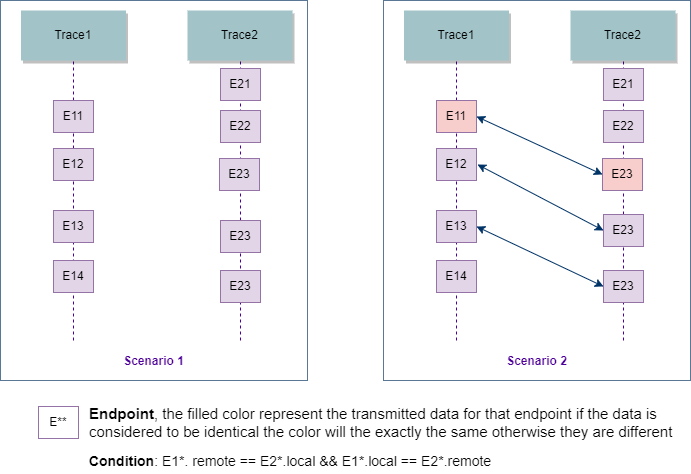
\includegraphics[scale=0.55]{Figures/channelreusetcpudp}}
 \caption{Channel Reuse Scenarios}
\label{communicationhappen}
\end{figure}

\begin{algorithm}[H]
\DontPrintSemicolon
\caption{{\bf Channel Indentification Algorithm for TCP and UDP} \label{channelAlg1}}
\KwIn{two endpoint lists of the dual-trace}
\KwOut{channel list}
$channels \leftarrow Map \langle String, List \langle Channel \rangle \rangle$;\; 
\For{$endpoint \in endpointList1$}{
   $openEvent1 \leftarrow$ get the event from $endpoint.openStream$, which should only contain one event. 
   $channelId1 \leftarrow$ get the channel identifier from $openEvent1.inputs$;\;
   \For{$endpoint2 \in endpointList2$}{
      $openEvent2 \leftarrow$ get the event from $endpoint2.openStream$, which should only contain one event.
      $channelId2 \leftarrow$ get the channel identifier from $openEvent2.inputs$;\;
    \If{$channelId1 == channelId2$}{
       $channel = New \enspace Channel()$;\;
       $channels.add\left( channel \right)$;\;
    }
   }
}
\KwRet $channels$;\;
\end{algorithm}

\subsection{Transported Stream Data Verification}

\subsection{Transported Event Data Verification}

\subsection{Data Structure for Identified Communications}

\section{Communication Identification Feature Prototype}

	\externaldocument{../3/chapter_modeling}
\externaldocument{../4/chapter_algorithm}
\startchapter{Dual\_trace Communication Analysis Prototype On Atlantis}
\label{chapter:newsol}
In this chapter, I present the design of the prototype of communication analysis from the dual\_trace. This prototype is implemented on Atlantis. Atlantis as an assembly execution trace analysis environment. It provides many features that benefit the communication analysis of dual\_trace. 

This prototype consists of four components: 1) declaring the function descriptors of the communication methods. 2) a view that can display both traces in the dual\_trace in parallel. 3)implementation of the communication analysis algorithms for stream extraction and communication identification. 4) a view for presenting the extracted streams and the identified communications from the dual\_trace.

\section{Use Case}
In this section, the use cases are presented to depict how to use the developed components and the existing features of Atlantis to perform the communication analysis.

To analyze a dual\_trace, the user need to perform the below operations in sequence:
\begin{itemize}
\item Open two traces in the parallel view (as part of this prototype)
\item Import the dynamic linked library files for each trace (as part of existing functionality of Atlantis)
\item Perform the stream extraction or communication identification operations(as part of this prototype)
\item Inspect the operation results by navigating the analysis result from the communication view (as part of this prototype).
\end{itemize}

Two use cases of this prototype are designed. The use case shown in Table \ref{usecase1} is for stream extraction and the use case shown in Table \ref{usecase2} is for communication identification. 

\begin{table}[H]
  \centering
  \caption{Use Case 1: Extract Streams from the Dual\_trace}
  \label{usecase1}
  \begin{tabular}{|l|p{13cm}|}
      \hline
       \textbf{Name} & Analysis streams of a communication method from the Dual\_trace\\
       \hline
       \textbf{Description} & A user captured two assembly execution traces of two interacting programs and needs to analysis them by extracting all communication streams of each of the traces and inspecting the extraction results \\
       \hline
              \textbf{Actor} & A Software Security Engineer \\
       \hline
       \textbf{Precondition} & The user has two assembly execution traces and the .dll files of the systems where the programs of the captured traces were running\\
       \hline
       \textbf{Main Course}& 1. The user declares the function descriptors for the communication methods of interest in a Json format setting file\\
        & 2. The user opens one of the trace in Atlantis\\
       &  3. The user opens the other trace as the dual\_trace of the first one\\
       & 4. The two opened traces are presented in the parallel view\\
       & 5. The user loads the related .dll files for both opened trace\\
       & 6. The user selects the operation ``Stream Extraction" in the ``Dual\_Trace Tool" menu.\\
       & 7. Atlantis prompts a dialog window giving the user all the communication methods in the function descriptor setting file as options\\
       & 8. The user selects the communication methods which they want to analyze and click the ``OK" bottom\\
       & 9. Atlantis extracts the streams for both traces and list the result in ``Communication view"\\
       & 10. The user expands the result in the ``Communication view"\\
       & 11. The user selects one function call event in a stream and double click the entry\\
       & 12. Atlantis shows the corresponding instruction line in the trace and synchronizes all other views\\
      \hline               
  \end{tabular}
\end{table}

\begin{table}[H]
  \centering
  \caption{Use Case 2: Identify Communications from the Dual\_trace}
  \label{usecase2}
  \begin{tabular}{|l|p{13cm}|}
      \hline
       \textbf{Name} & Identify communications of a communication method from the Dual\_trace\\
       \hline
       \textbf{Description} & A user captured two assembly execution traces of two interacting program and need to analysis them by identify all communications of the dual\_trace and inspecting the extraction results \\
       \hline
              \textbf{Actor} & A Software Security Engineer \\
       \hline
      \textbf{Precondition} & The user has two assembly execution traces and the .dll files of the systems where the programs of the captured traces were running\\
       \hline
       \textbf{Main Course}& 1. The user declares the function descriptors for the communication methods of interest in a Json format setting file\\
        & 2. The user opens one of the trace in Atlantis\\
       &  3. The user opens the other trace as the dual\_trace of the first one\\
       & 4. The two opened traces are presented in the parallel view\\
       & 5. The user loads the related .dll files for both opened trace\\
       & 6. The user selects the operation ``Communication Identification" in the ``Dual\_Trace Tool" menu\\
      & 7. Atlantis prompts a dialog window giving the user all the communication methods in the function descriptor setting file as options\\
       & 8. The user selects the communication methods which they want to analyze and click the ``OK" bottom\\
       & 9. Atlantis identifies the communications of the dual\_trace and list the result in ``Communication view"\\
       & 10. The user expands the result in the ``Communication view"\\
       & 11. The user selects one function call event in a stream and double click the entry\\
       & 12. Atlantis shows the corresponding instruction line in the trace and synchronize all other views\\
      \hline               
  \end{tabular}
\end{table}

\section{Declaring of the Function Descriptors}\label{functionset}
In Section \ref{cdesc}, I describe how to define a function descriptor for each communication method. Each function description consist with four elements: 

$fdesc = \lbrace name, type, inparamdesc, outparamdesc \rbrace$

$name$ is the function name, $type$ can be $open$, $close$, $send$ and $receive$, $inparamdesc$ and $outparamdesc$ are the descriptions for the input and output parameters of interest(we might not care for all parameters). The communication analysis approach depicted in Chapter \ref{chapter:alo} can identify the communications described by the function descriptor from the dual\_trace.

However, the function descriptor for a communication method can be different depending on the implementation of the communication method in a program. Rather than hard coding the function descriptors for the communication methods, the prototype loads the function descriptors from a configuration file. A default template is given for reference. This template is generated by Atlantis when it is launched and stored in the .tmp folder of the trace analysis project. The users can modify this template as to the communication methods of interest. The default template example can be found in Appendix \ref{funcset}.

The function descriptors in this configuration file will be the input for the stream extraction and communication identification features. When the user uses these two features, the list of the communication methods provided in the function descriptor configuration file will be presented to them. They can select one or more communication methods to be analyzed. 

In the following subsections, function descriptor examples are presented for reference. Other function descriptors can be created by following the same method as developing the function descriptor examples.

\subsection{Communication Methods' Implementation in Windows}\label{windows}
Learning the implementation of a communication is necessary to obtain the function descriptor of the communication method. In this section, I present the results of analyzing the implementation of these four communication methods: Named Pipe, Message Queue, TCP and UDP in Windows. In the analysis, I reviewed the Windows APIs of the communication methods and their example code. By doing so, I obtained the function descriptors of these methods. 

The Windows API set is very complex. Moreover, multiple solutions are provided to fulfil a communication method. It is unfeasible within the scope of this thesis to enumerate all solutions for each communication method. I only investigated the most basic usage provided in Windows documentation. For each communication method, a function descriptor with a list of system function descriptions is provided for reference. The functions in the descriptors are supported in most Windows operating systems, such as Windows 8, Window 7. The provided function descriptor of a communication method should only be considered as an example for that communication method. With the understanding of this, it should be fairly easy to obtain the function descriptors for other solutions of that communication method or other communication methods. 

Note that, the instances of the descriptors only demonstrate Windows C++ APIs. But the idea of the function descriptor is generalizable to other operating systems with the effort of understanding the APIs of those operating systems.

\subsubsection{Windows Calling Convention}
Ror this research, it is important to know the Windows calling convention. The communication analysis from a dual\_trace in assembly level relies not only on the system function names but also the key parameter values and return values. In the assembly level execution traces, the parameter and return values are captured in the memory changes and register changes of the instructions but without any explicit information indicating which registers or memory addresses are holding these parameters. The calling convention tells us where the parameters are stored. So that, we can find them in the memory state while emulating the execution of the trace. Each operating system has their own calling convention for different programming languages. I used dual\_traces of Microsoft* x64 programs for case study in this research. The Microsoft* x64 calling convention is listed in Appendix \ref{convention} for reference.

\subsubsection{Named Pipes}
In Windows, a named pipe is a communication method between one server and one or more clients. The pipe has a name and can be one-way or duplex. Both the server and clients can read or write into the pipe\cite{WinNamedpipe}. In this work, I only consider one server versus one client communication (one server to multiple clients scenario can always be divided into multiple ``one server and one client" communications thanks to the characteristic that each client and server communication has a separate conduit). The server and client are endpoints in the communication. We call the server ``server endpoint" and the client ``client endpoint".  The server endpoint and client endpoint of a named pipe share the same pipe name, but each endpoint has its own buffers and handles. 

There are two modes for data transfer in the named pipe communication method, synchronous and asynchronous. Modes affect the functions used to complete the send and receive operations. The function descriptors for both synchronous mode and asynchronous mode are provided. The create channel functions for both modes are the same while the mode is indicated by an input parameter. The functions for send and receive message are also the same for both cases. However, the operations of the send and receive functions are different for different modes. In addition, an extra function \textit{GetOverlappedResult} is being called to check if the sending or receiving operation finished, the output message will be stored in the overlap structure whose memory address saved in the function's output parameter OverlapStruct. Table \ref{namesyn} is the function descriptor for synchronous mode while Table \ref{nameasyn} is the function descriptor asynchronous mode of Named pipe.

\begin{table}[H]
  \centering
  \caption{Function Descriptor for Synchronous Named Pipe}
  \label{namesyn}
  \begin{tabular}{|l|l|l|l|l|l|l|l|}
\hline
             \multirow{2}{*}{{\textbf{Name}}} & \multirow{2}{*}{{\textbf{Type}}} & \multicolumn{3}{c|}{\textbf{Input Parameters Description}} & \multicolumn{3}{c|}{\textbf{Output Parameters Description}} \\
              \cline{3-8} 
             & & \textbf{Name}& \textbf{Register} & \textbf{Addr/Val} & \textbf{Name}& \textbf{Register} &  \textbf{Addr/Val}  \\
             \hline
      CreateNamedPipe
       &open & FileName & RCX  & Addr &  Handle & RAX & Val\\
      \hline         
      CreateFile
       &open & FileName & RCX & Addr&  Handle & RAX & Val\\ 
      \hline              
      \multirow{2}{*}{WriteFile}
       &\multirow{2}{*}{send} &  Handle & RCX & Val & Length & R9 &Val\\
        \cline{3-8} 
       & & SendBuf & RDX & Addr & RetVal& RAX & Val\\
      \hline            
      \multirow{2}{*}{ReadFile}
       &\multirow{2}{*}{receive} &  Handle & RCX & Val& Length &R9 & Val\\
        \cline{3-8} 
       & & RecvBuf & RDX  & Addr & RetVal& RAX & Val\\
      \hline            
      CloseHandle &
       close &  Handle & RCX & Val & RetVal& RAX & Val\\
      \hline            
      DisconnectNamedPipe &
      close &  Handle & RCX & Val & RetVal& RAX & Val\\
      \hline               
  \end{tabular}
\end{table}

\begin{table}[H]
  \centering
  \caption{Function Descriptor for Asynchronous Named Pipe}
  \label{nameasyn}
\begin{tabular}{|l|l|l|l|l|l|l|l|}
\hline
             \multirow{2}{*}{{\textbf{Name}}} & \multirow{2}{*}{{\textbf{Type}}} & \multicolumn{3}{c|}{\textbf{Input Parameters Description}} & \multicolumn{3}{c|}{\textbf{Output Parameters Description}} \\
              \cline{3-8} 
             & & \textbf{Name}& \textbf{Register} & \textbf{Addr/Val} & \textbf{Name}& \textbf{Register} &  \textbf{Addr/Val}  \\
             \hline
      CreateNamedPipe
       &open & FileName & RCX  & Addr &  Handle & RAX & Val\\
      \hline         
      CreateFile
       &open & FileName & RCX & Addr&  Handle & RAX & Val\\ 
      \hline              
      \multirow{2}{*}{WriteFile}
       &\multirow{2}{*}{send} &  Handle & RCX & Val & Length & R9 & Val\\
        \cline{3-8} 
       & & SendBuf & RDX & Addr & RetVal& RAX & Val\\
      \hline            
      \multirow{2}{*}{ReadFile}
       &\multirow{2}{*}{receive} &  Handle & RCX & Val& Length & R9 & Val\\
        \cline{3-8} 
       & & RecvBuf & RDX  & Addr & RetVal& RAX & Val\\
      \hline    
           \multirow{2}{*}{GetOverlappedResult} &
       \multirow{2}{*}{receive} &  \multirow{2}{*}{Handle} & \multirow{2}{*}{RCX} & \multirow{2}{*}{Val} &OverlapStruct &RDX & Addr\\
               \cline{6-8} 
       & &  &   &  & RetVal& RAX & Val\\
      \hline     
      CloseHandle &
       close &  Handle & RCX & Val & RetVal& RAX & Val\\
      \hline            
      DisconnectNamedPipe &
      close &  Handle & RCX & Val & RetVal& RAX & Val\\
      \hline               
  \end{tabular}  
\end{table}

\subsubsection{Message Queue}
Similar to Named Pipe, the Message Queue's implementation in Windows also has two modes, synchronous and asynchronous. The asynchronous mode is also further divided into two operations: one with callback function and the other without. With the callback function, the callback function would be called when the send or receive operations finish. Without a callback function, the general function \textit{MQGetOverlappedResult} should be called by the endpoints to check if the message sending or receiving operation finish, the parameter in RCX of this function call is a structure consist of the handle as an input parameter and the overlap structure as an output parameter. Table \ref{msmqsynfunctions} is the function descriptor for synchronous mode while Table \ref{msmqasynfunctions} is the function descriptor for the asynchronous mode without callback. I did not exemplify the case the with callback function, since the specific callback function and its parameters need to be known for developing this the function descriptor.

\begin{table}[H]
  \centering
  \caption{Function Descriptor for Synchronous Message Queue}
  \label{msmqsynfunctions}
\begin{tabular}{|l|l|l|l|l|l|l|l|}
\hline
             \multirow{2}{*}{{\textbf{Name}}} & \multirow{2}{*}{{\textbf{Type}}} & \multicolumn{3}{c|}{\textbf{Input Parameter Description}} & \multicolumn{3}{c|}{\textbf{Output Parameter Description}} \\
              \cline{3-8} 
             & & \textbf{Name}& \textbf{Register} & \textbf{Addr/Val} & \textbf{Name}& \textbf{Register} &  \textbf{Addr/Val}  \\
             \hline
      MQOpenQueue
       &open & QueueName & RCX  & Addr &  Handle & RAX & Val\\
      \hline                     
      \multirow{2}{*}{MQSendMessage}
       &\multirow{2}{*}{send} &  Handle & RCX & Val & \multirow{2}{*}{RetVal} & \multirow{2}{*}{RAX}  & \multirow{2}{*}{Val} \\
       \cline{3-5}
      & & MessStruct& RDX&Addr &   &  &  \\
      \hline            
      \multirow{2}{*}{MQReceiveMessage}
       &\multirow{2}{*}{receive}&  \multirow{2}{*}{Handle} & \multirow{2}{*}{RCX} & \multirow{2}{*}{Val}& MessStruct& RDX&Addr\\
              \cline{6-8}
      & & & & & RetVal & RAX & Val\\
      \hline       
      MQCloseQueue &
       close &  Handle & RCX & Val & RetVal & RAX & Val\\
      \hline                          
  \end{tabular}   
\end{table}

\begin{table}[H]
  \centering
  \caption{Function Descriptor for Asynchronous Message Queue}
  \label{msmqasynfunctions}
\begin{tabular}{|l|l|l|l|l|l|l|l|}
\hline
             \multirow{2}{*}{{\textbf{Name}}} & \multirow{2}{*}{{\textbf{Type}}} & \multicolumn{3}{c|}{\textbf{Input Parameter Description}} & \multicolumn{3}{c|}{\textbf{Output Parameter Description}} \\
              \cline{3-8} 
             & & \textbf{Name}& \textbf{Register} & \textbf{Addr/Val} & \textbf{Name}& \textbf{Register} &  \textbf{Addr/Val}  \\
             \hline
      MQOpenQueue
       &open & QueueName & RCX  & Addr &  Handle & RAX & Val\\
      \hline                     
      \multirow{2}{*}{MQSendMessage}
       &\multirow{2}{*}{send} &  Handle & RCX & Val & \multirow{2}{*}{RetVal} & \multirow{2}{*}{RAX}  & \multirow{2}{*}{Val} \\
       \cline{3-5}
      & & MessStruct& RDX&Addr &   &  &  \\
      \hline            
           \multirow{2}{*}{MQReceiveMessage}
       &\multirow{2}{*}{receive}&  \multirow{2}{*}{Handle} & \multirow{2}{*}{RCX} & \multirow{2}{*}{Val}& MessStruct& RDX&Addr\\
              \cline{6-8}
      & & & & & RetVal & RAX & Val\\
      \hline    
      \multirow{2}{*}{MQGetOverlapResult} &
       \multirow{2}{*}{receive} &  \multirow{2}{*}{Handle} & \multirow{2}{*}{RCX} & \multirow{2}{*}{Addr} & Overlapstr& RCX&Addr\\
                     \cline{6-8}
      & & & & & RetVal & RAX & Val\\
      \hline      
      MQCloseQueue &
       close &  Handle & RCX & Val & RetVal & RAX & Val\\
      \hline                          
  \end{tabular}   
\end{table}


    
\subsubsection{TCP and UDP}
In Windows programming, these two methods share the same set of APIs regardless of whether the input parameter values and operation behavior are different. In the Windows socket solution, one of the two endpoints is the server while the other one is the client. Table \ref{tcpupdfunctions} is the function descriptor for UDP or TCP communication. 

\begin{table}[H]
  \centering
  \caption{Function Descriptor for for TCP and UDP}
  \label{tcpupdfunctions}
\begin{tabular}{|l|l|l|l|l|l|l|l|}
\hline
             \multirow{2}{*}{{\textbf{Name}}} & \multirow{2}{*}{{\textbf{Type}}} & \multicolumn{3}{c|}{\textbf{Input Parameters Description}} & \multicolumn{3}{c|}{\textbf{Output Parameters Description}} \\
              \cline{3-8} 
             & & \textbf{Name}& \textbf{Register} & \textbf{Addr/Val} & \textbf{Name}& \textbf{Register} &  \textbf{Addr/Val}  \\
             \hline
      socket
       &open &  &   &  &  Socket & RAX & Val\\ 
      \hline
      bind
       &open & Socket &  RCX & Val &  ServerAddrAndPort & RDX & Addr\\
      \hline   
            connect
       &open & Socket &  RCX & Val &  ServerAddrAndPort & RDX & Addr\\
      \hline   
     accept
       &open &  ListenSocket & RCX & Val & ConnectSocket & RAX & Val\\
      \hline                    
      \multirow{2}{*}{send}
       &\multirow{2}{*}{send} &  Handle & RCX & Val & \multirow{2}{*}{RetVal}& \multirow{2}{*}{RAX} & \multirow{2}{*}{Val} \\
       \cline{3-5}
      & & SendBuf& RDX&Addr &  &  & \\
      \hline            
      \multirow{2}{*}{recv}
       &\multirow{2}{*}{receive}&  \multirow{2}{*}{Handle} & \multirow{2}{*}{RCX} & \multirow{2}{*}{Val}& RecvBuf& RDX&Addr\\
       \cline{6-8}
      & &  &   &  &  RetVal & RAX & Val\\ 
      \hline      
      closesocket &
       close &  Handle & RCX & Val & RetVal & RAX & Val\\
      \hline                          
  \end{tabular}    
\end{table}

\section{Parallel Trace View For Dual\_Trace}
The dual\_trace consists of two execution traces which are interacting with each other. I have implemented a view that shows the traces side by side. It's called the parallel trace view. Presenting two traces in the parallel trace view makes the analysis for the user much easier. A parallel trace view implemented in Atlantis can display two execution traces side by side. To open the parallel trace view, the user needs to open one trace as the normal one and the other as the dual\_trace of the active (opened) one. A new menu option in the project navigation view of Atlantis was added to open the second trace as the dual\_trace of the active one. The implementation of the parallel view takes advantage of the existing SWT of Eclipse plug-in development. The detail of the implementation can be found in Appendix \ref{parallelview}. Figure \ref{opendualtracemenu} shows the ``Open as Dual\_Trace" menu option and Figure \ref{parallelview} shows the parallel trace view with two traces displaying side by side.

\begin{figure}[H]
\centerline{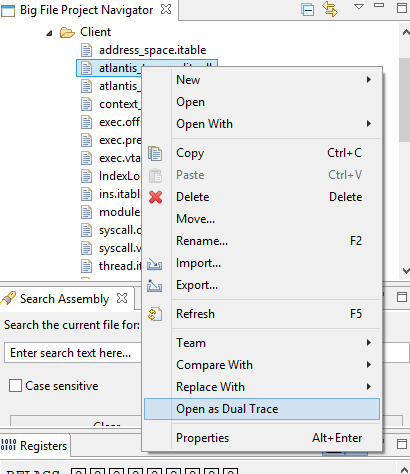
\includegraphics[scale=0.4]{Figures/opendualtracemenu}}
 \caption{Menu Item for opening Dual\_trace}
\label{opendualtracemenu}
\end{figure}

\begin{figure}[H]
\centerline{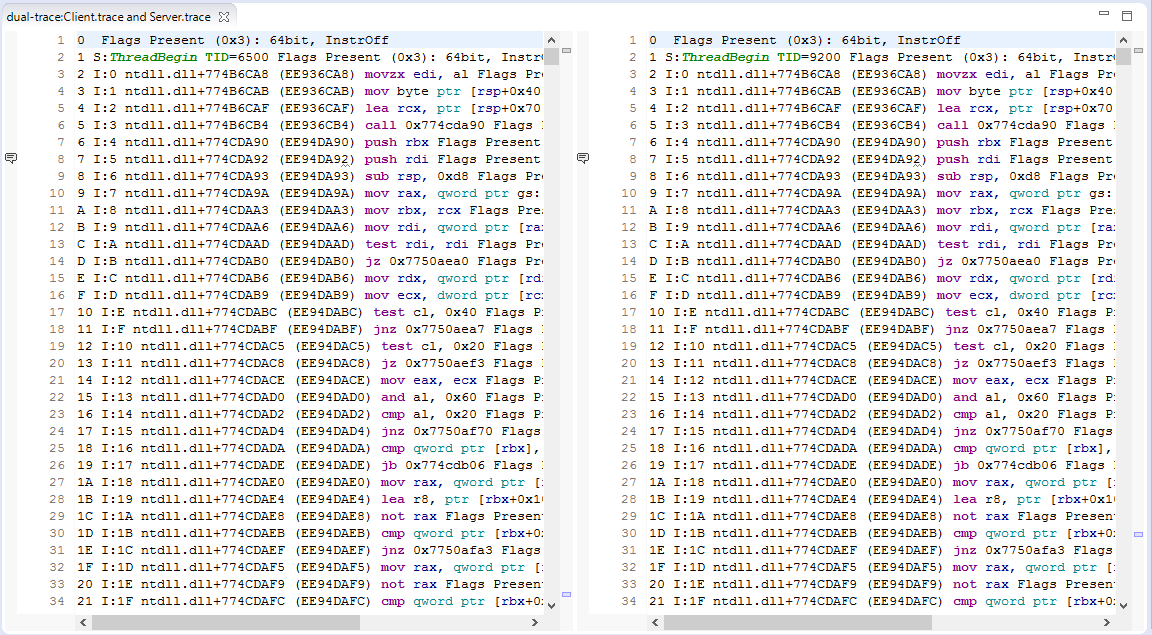
\includegraphics[scale=0.6]{Figures/paralleleditor}}
 \caption{Parallel Trace View}
\label{parallelview}
\end{figure}

\section{Implementation of the Communication Analysis Algorithms}
The implementation is divided into two parts. The first part is the stream extraction. It implements the first section of the overall process of the communication analysis as shown in the left side of Figure \ref{overviewintwo} and presents the extracted streams of both traces in the dual\_trace to the user. The second part is the communication identification. It implements the whole process of the communication analysis as shown in the right side of Figure \ref{overviewintwo} and presents the identified communications of the dual\_trace to the user.

\begin{figure}[H]
\centerline{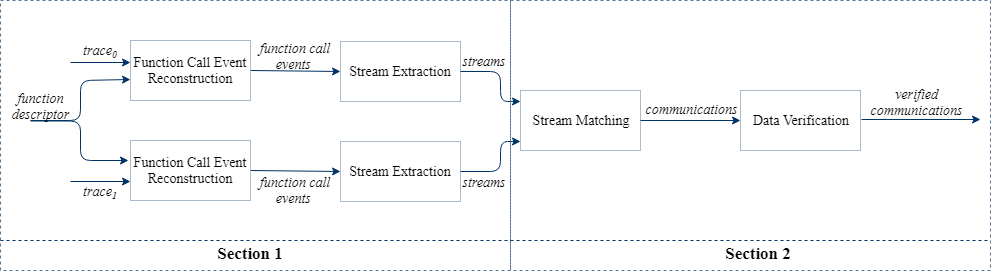
\includegraphics[scale=0.55]{Figures/overviewintwo}}
\caption{Process of the Communication Analysis from a Dual\_trace Separated in Two Sections}
\label{overviewintwo}
\end{figure}

<<<<<<< HEAD
The implementation relies on the existing ``function inspect" feature of Atlantis. The called functions' name can be inspected  by  searching of the symbolic name in the executable binary or any DLLs which used by the program at the time when it is traced. By importing the DLLs and executable binary, Atlantis can recognize the function call from the execution trace using the function names. Therefore the corresponding Dlls or executable binaries for both traces in the dual\_trace have to be loaded into Atlantis before conducting these two operations.

A new menu ``Dual\_trace Tool" with three menu options is designed for these two operations. In this menu, ``Stream Extraction" is for the operation of stream extraction and ``Communication Identification" is for the operation of communication identification. Before performing both of these two operation, ``Load Library Exports" has to be run for both traces. Currently, the ``Load library export"  operation can only load libraries for the trace in the active trace view. So ``Load library export"  in the menu has to be run twice separately for each trace of the dual\_trace.  Figure \ref{dualtracetoolmenu} shows this new menu in Atlantis. When the user perform ``Stream Extraction" or ``Communication Identification", there will be a prompt dialog window as shown in Figure \ref{methods} which asks the user what communication methods they want to analyze from the dual\_trace. This list is provided by the configuration file I mention in Section \ref{functionset}. The user can select one or multiple methods. Atlantis will perform the operations after the user selects and confirms the communication methods.
=======
The format of the traces I got from DRDC for this research is slightly different from the formulation of the trace in Section \ref{dualtrace}. In stead of having the function name in $syscallInfo$, the current traces only provide the offset of that function in the corresponding executable file. So that, the trace needs to be processed to comply with the trace formalization.
The existing ``function inspect" feature of Atlantis can provide this pre-processing functionality. The called functions' name can be inspected  by  search of the symbolic name in the executable binary or any DLLs which used by the program at the time when it is traced. Figure \ref{trace} is an example of the trace from DRDC. In this example, line 1504 is a system call entry with the system call info as $syscallInfo = <kernal32.dll, 0x10D10>$. 
Figure \ref{executable} is the information decoded by the ``function inspect" feature of Atlantis from the executable file kernal32.dll of the system where the trace shown in Figure \ref{trace} was captured. So that the instruction line 1504 is a system call entry of $CreateFileW$. By loading a .dll file (in this case kernel32.dll) for the trace, Atlantis can translate system call information in the current trace format the one align to the dual\_trace formalization.

\begin{figure}[H]
\centerline{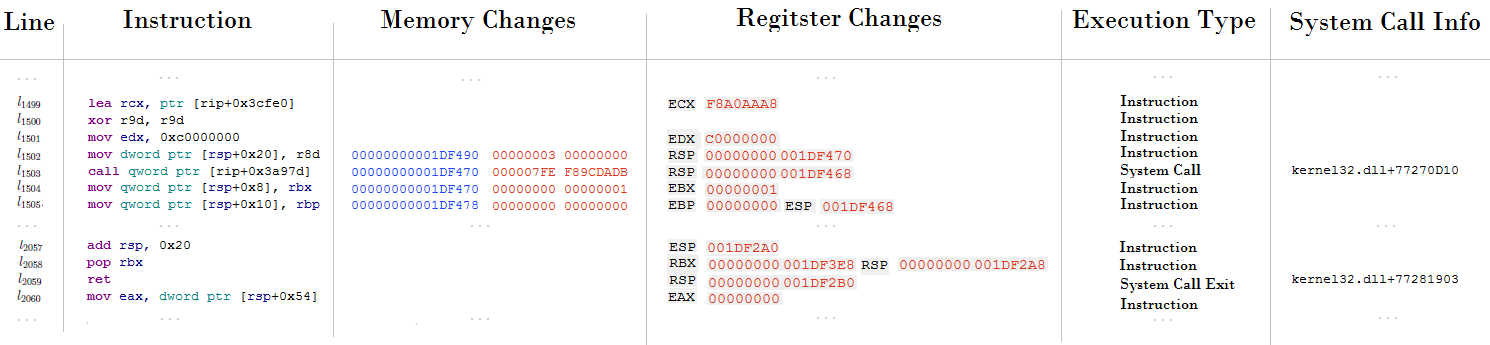
\includegraphics[scale=0.45]{Figures/trace}}
\caption{An example trace from DRDC}
\label{trace}
\end{figure}

\begin{figure}[H]
\centerline{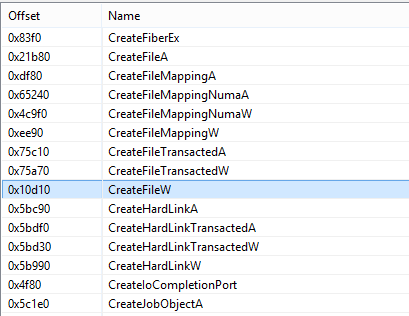
\includegraphics[scale=0.6]{Figures/executable}}
\caption{Information from kernal32.dll}
\label{executable}
\end{figure}

A new menu ``Dual\_trace Tool" with three menu options is designed for these two operations. In this menu, ``Stream Extraction" is for the operation of stream extraction and ``Communication Identification" is for the operation of communication identification. Before performing both of these two operation, ``Load Library Exports" has to be run for both traces. ``Load Library Exports" option in this menu triggers the ``function inspect" operation for the active trace. After this operation being run separately for both traces in the dual\_trace. The traces are transformed into the proper format for communication analysis. Figure\ref{dualtracetoolmenu} shows this new menu in Atlantis. When the user perform ``Stream Extraction" or ``Communication Identification", there will be a prompt dialog window as shown in Figure \ref{methods} which asks the user what communication methods they want to analyze from the dual\_trace. This list is provided by the configuration file I mentioned in Section \ref{functionset}. The user can select one or multiple methods. Atlantis will perform the operations after the user select and confirm the communication methods.

\begin{figure}[H]
\centerline{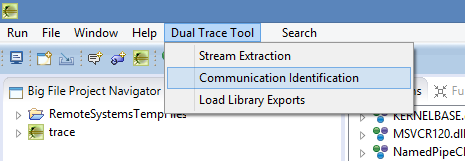
\includegraphics{Figures/dualtracetoolmenu}}
 \caption{Dual\_trace Tool Menu}
\label{dualtracetoolmenu}
\end{figure}

\begin{figure}[H]
\centerline{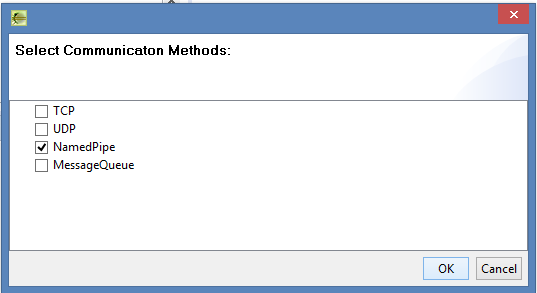
\includegraphics[scale=0.8]{Figures/methods}}
 \caption{Prompt Dialog for Communication Selection}
\label{methods}
\end{figure}


\section{View of Extracted Streams and Identified Communications}
A new view named ``Communication View" is designed for presenting the result of the extracted streams and the identified communications. Since the user might have selected multiple selection for communication methods of interest, the output result contains all the streams or communications of all selected communication methods and the results are clustered by methods. There are two sub tables in this view, the left one is for presenting the extracted streams while the left one is for presenting identified communications. The reason for putting these two results in the same view is for easy access to and comparison of the data for the users. Figure \ref{idenview} shows this view with both extracted stream results and identified communication results in it. Each time when the user reruns the operations the result in the corresponding table will be refreshed to show only the latest result of that operation. But the other table will not be affected. For example, if the user run the ``Stream Extraction" operation first, the extracted streams will be shown on the left table of the view. And then if the user performs the ``communication Identification" operation, the identified communications result will be shown on the right table while the left one still holds the last stream extraction result.

\begin{figure}[H]
\centerline{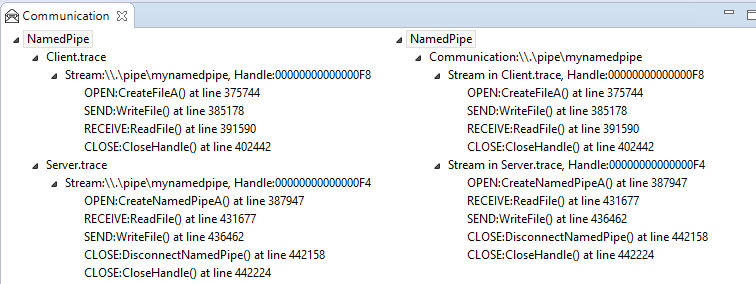
\includegraphics[scale=0.7]{Figures/idenview}}
 \caption{Communication View for Result}
\label{idenview}
\end{figure}

Atlantis is a analysis environment that has various views to allow user access to different information from the trace, such as the memory and register state of the current instruction line. Moreover, these views synchronize automatically with the trace view. These functionality and information also benefit the communication analysis of the dual\_trace. Providing the user a way to navigate from the result of the extracted streams and the identified communications to the trace views allows them to take advantage of the current existing functionality of Atlantis and make their analysis of the dual\_trace more efficient.

The results presented in the Communication view contains all the function call events. The memory state at the instruction line of the function begin contains the input parameters and the memory state at the instruction line of the function return contains the output parameters and the return value. In order to provide the user an method to easily access these two instruction lines, from the event entries, this implementation provide two different ways for the user to navigate back to where the function begins and ends. When the user ``double clicks" on an entry, it will bring the user to the start line of the function in the corresponding trace view. When the user right clicks on the event entry, a prompted menu with the option ``Go To Line of Function End" will show up as shown in Figure \ref{gotoend}. Clicking on this option will bring the user to the return line of this function in the trace view. All other opened views of Atlantis update immediately with this navigation. By these navigations, the users can easily see the sent and received message of the events.

\begin{figure}[H]
\centerline{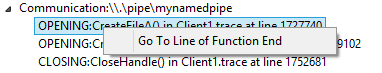
\includegraphics{Figures/gotoend}}
 \caption{Right Click Menu on Event Entry}
\label{gotoend}
\end{figure}

Moreover, the ``remove" option, as shown in Figure \ref{remove}, in the right click menu on the ``stream“ or ``communication" entries is provided for the user to remove the selected ``stream" or ``communication" entry. This provides the users the flexibility to get rid of data that they are not interested about.

\begin{figure}[H]
\centerline{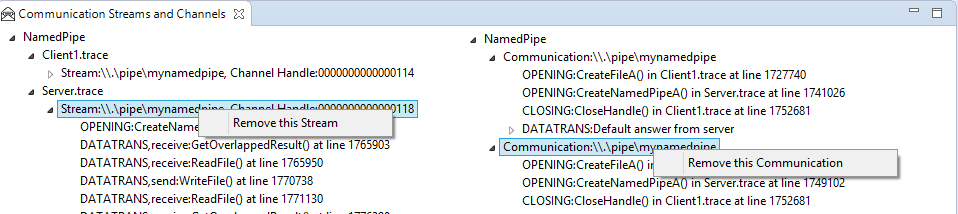
\includegraphics[scale=0.7]{Figures/remove}}
 \caption{Right Click Menu on Event Entry}
\label{remove}
\end{figure}


	\externaldocument{../appendix/chapter_app}
\externaldocument{../4/chapter_algorithm}
\externaldocument{../3/chapter_modeling}
\startchapter{Proof of Concept}
\label{chapter:Exp}
In this section, I present two experiments I ran for the proof of concept of the communication analysis though execution traces.

These experiments aimed to test the communication model and the communication identification approach. They also verify the design of the some algorithms, for their correctness.  

User case study is not included in this thesis and can be the future work. The feature prototype implementation is not evaluated and can be part of the user case study. But I used the implemented feature on Atlantis to conduct the experiments.

I first present the design of the experiments and their result. And then, I discuss the result of the experiments.  

\section{Experiments}
In this section, I describe the design of the experiments. Two experiments are conducted in this research. All test programs in these two experiments were written in C++ and the source code can be found in Appendix \ref{expcode}. Our research partner DRDC executed the programs in their environment and provided the captured traces, the used .dll files and the source code of the programs for the experiments.

Results are provided for each experiment. Both of the conducted experiments were about named pipe communication method. The following two subsections provides the details of the experiments and their result.

\subsection{Experiment 1}
In the first experiment, two programs communicated with each other through a synchronous Named pipe channel. One of the programs acted as the Named pipe server while the other as the client. Figure \ref{exp1} is the sequence diagram of the interaction between the server and client. Traces were captured while these two program were running and interacting. The two captured traces were analysed as dual\_trace $exp1$ in this experiment. I used the implemented features in Atlantis to analyse this dual\_trace. I ran the ``Stream identification" and ``Communication identification" operations for this dual\_trace. The streams and communication are showed in Figure\ref{result1}.

\begin{figure}[H]
\centerline{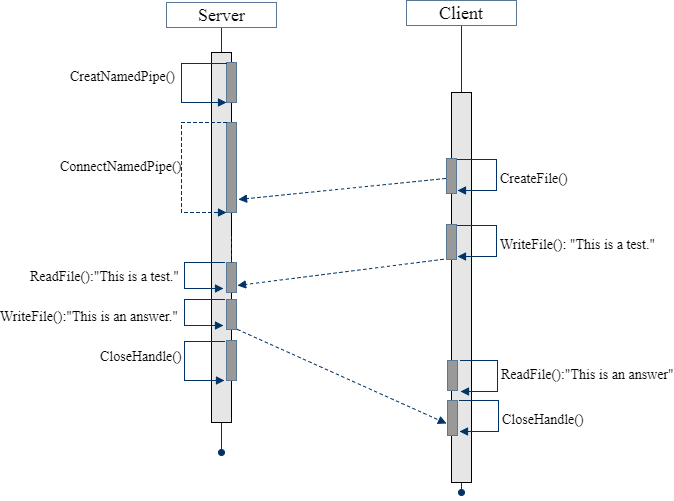
\includegraphics[scale=0.7]{Figures/exp1}}
 \caption{Sequence Diagram of Experiment 1}
\label{exp1}
\end{figure}

\begin{figure}[H]
\centerline{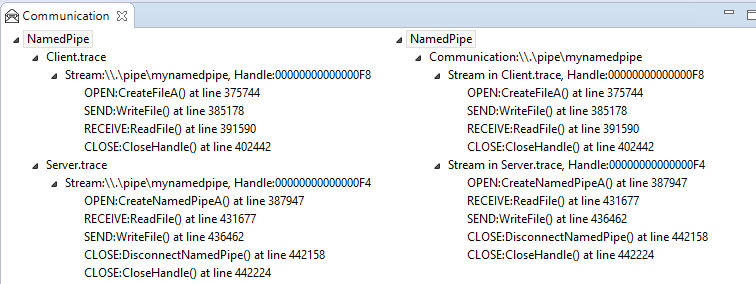
\includegraphics[scale=0.65]{Figures/result1}}
 \caption{Identification result of $exp1$}
\label{result1}
\end{figure}

\subsection{Experiment 2}
In the second experiment, one program was running as the Named pipe server. In this server program, four named pipes were created and can be connected by up to four client at a time. Two other programs as the Named pipe clients connected to this server. Those two clients (client 1 and client 2) used the identical program but run in sequence. Figure \ref{exp2} is the sequence diagram of the interaction among the server and clients. The function calls' sequence is only a possible combination from analyzing the source code. The real happening sequence can varies. Traces were captured at the time when these three programs were running and interacting. One trace for each program. The three traces are analysed as two dual\_traces, $exp2.1$ and $exp2.2$. $exp2.1$ consists of traces of server and client 1 and $exp2.2$ consists of traces of server and client 2. I ran the ``Stream identification" and ``Communication identification" operations for these two dual\_trace. The identified streams and communications are shown in Figure \ref{result21} and Figure \ref{result22}.

\begin{figure}[H]
\centerline{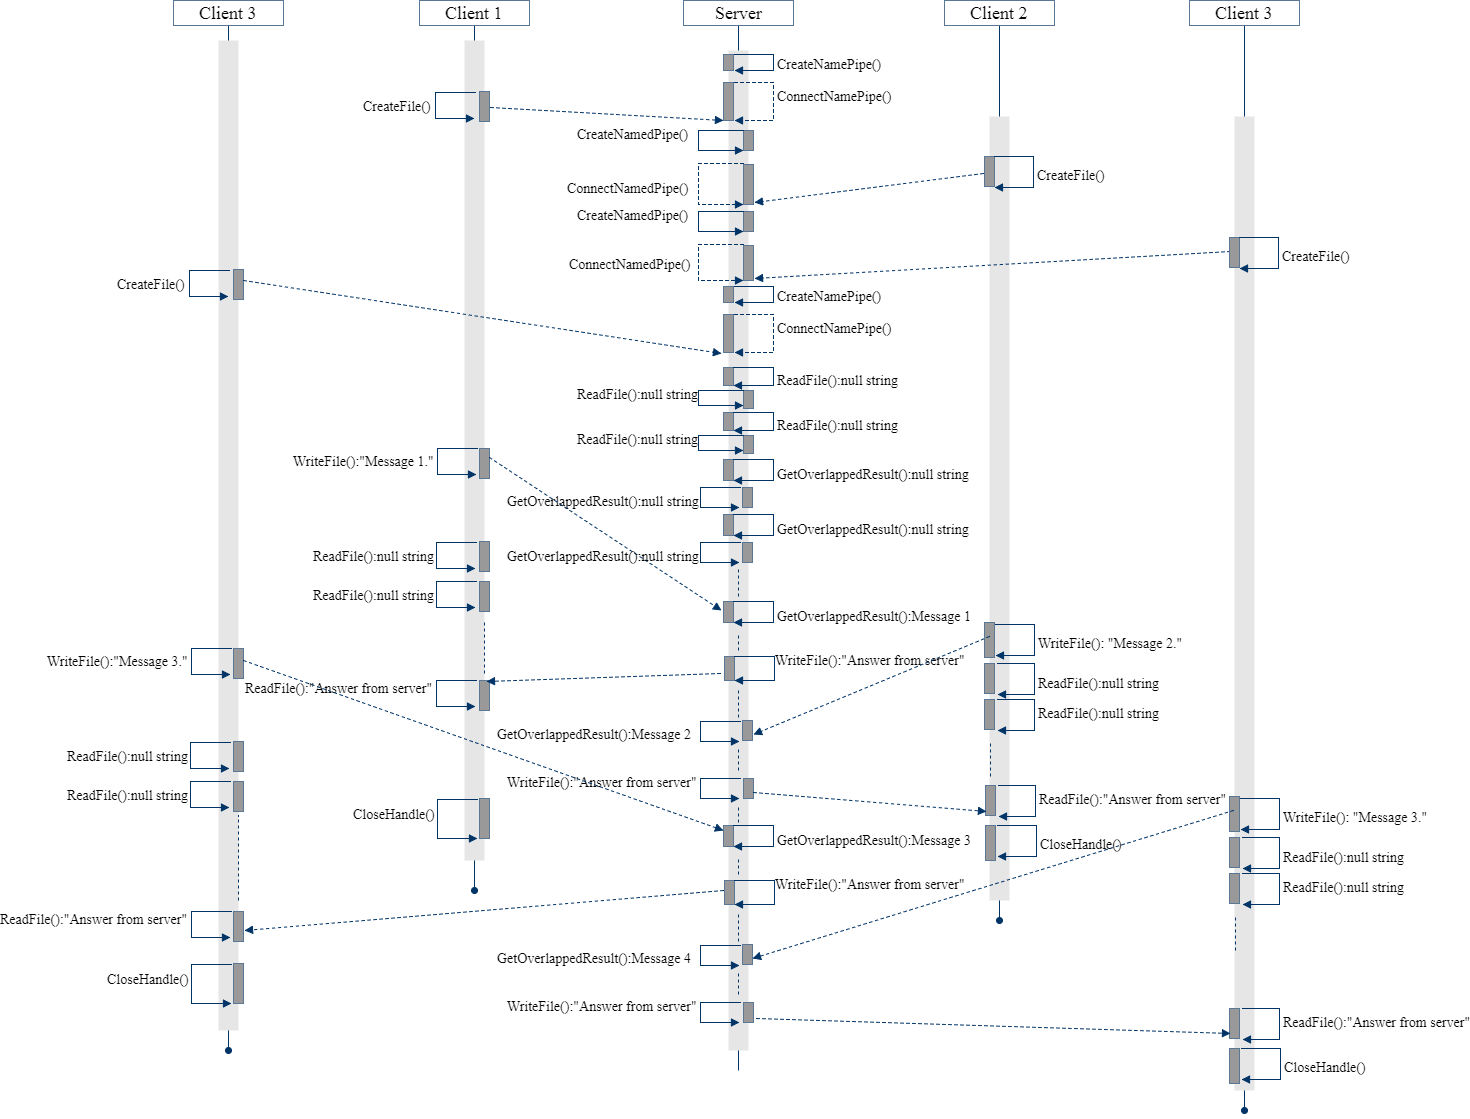
\includegraphics[scale=0.6]{Figures/exp2}}
 \caption{Sequence Diagram of Experiment 2}
\label{exp2}
\end{figure}

\begin{figure}[H]
\centerline{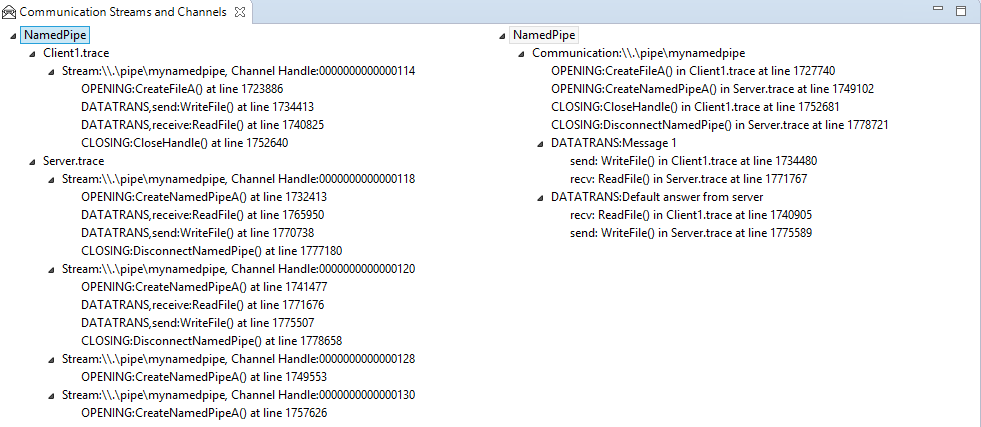
\includegraphics[scale=0.55]{Figures/result21}}
 \caption{Identification result of $exp2.1$}
\label{result21}
\end{figure}

\begin{figure}[H]
\centerline{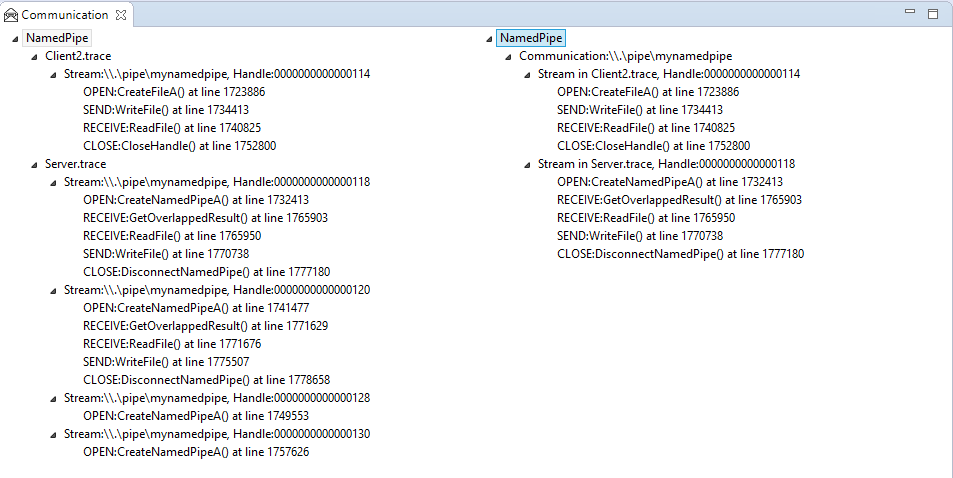
\includegraphics[scale=0.55]{Figures/result22}}
 \caption{Identification result of $exp2.1$}
\label{result22}
\end{figure}


\section{Discussion}
In the result of $exp1$, there are one stream extracted in client trace and one in server trace, and these two streams are matched into a communication of this dual\_trace. This identification result represents the actual communication happen between the named pipe server and client.
In the result of $exp2.1$ and $exp2.2$, there are one stream in each of the client traces and four in the server trace respectively. The streams are further matched and verified and eventually one communication is identified for each dual\_trace. The result aligns to the sequence diagram in Figure\ref{exp2}.


   





	\startchapter{Conclusions and Future Work}
\label{concl}
In this thesis, I present the approach of communication analysis through assembly level execution traces. I first defined the communication model. This abstract model depicts the outline of a communication between two running program, which gives the ground rule for the communication analysis. Then I depicted the general definition of the dual\_trace, the definition indicate that all traces comply to this definition can be used to conducted the communication analysis.

I also developed the essential algorithms for the communication identification. The high level algorithm is generalizable for all communication methods' identification while  the event stream extraction and matching algorithm are distinct for each communication method according to their channel open and data transfer mechanisms. However, the developed algorithms provides clear and referable examples to develop your own algorithm for communication methods which are not discussed in this thesis.

On top of the existing execution trace analysis environment Atlantis, I implemented the communication identification features. This feature provides the users a way to extend their concerned communication methods through the configuration file. The user interface allows the users to conduct the communication and stream identification from the dual\_traces and navigate back from the identified result to the views of the trace in Atlantis. This feature prototype is a novel feature for conducting multiple trace analysis for reverse engineering at the time when this thesis was written. The experiments conducted in this work preliminary proves the usability of the model and the algorithms. 

This thesis illustrates the novel idea and approach for dynamic program analysis which considerate the interaction of two programs. This idea is valuable due to the fact that programs or malware in the real world work collaboratively. The analysis of the communication and interaction of the programs provide more reliable information for vulnerability detection and program analysis.

Future work can be divided in two directions. One is extending the model to be more generalize for all kinds of interaction but not only the message transferring communications while the other is conducting user studies of the communication analysis approach and the feature design to get a more concrete result of their usefulness.


	\appendix
	\begin{appendices}	
\chapter{Microsoft x64 Calling Convention for C/C++}\label{convention}
\begin{itemize}  
\item RCX, RDX, R8, R9 are used for integer and pointer arguments in that order left to right.
\item XMM0, 1, 2, and 3 are used for floating point arguments.
\item Additional arguments are pushed on the stack left to right. \ldots 
\item Parameters less than 64 bits long are not zero extended; the high bits contain garbage.
\item Integer return values (similar to x86) are returned in RAX if 64 bits or less.
\item Floating point return values are returned in XMM0.
\item Larger return values (structs) have space allocated on the stack by the caller, and RCX then contains a pointer to the return space when the callee is called. Register usage for integer parameters is then pushed one to the right. RAX returns this address to the caller.
\end{itemize}

\chapter{Function Descriptor Configuration file Example}\label{funcset}
\lstinputlisting[caption= communicationMethods.json]{./sourcecode/communicationMethods.json}

\chapter{Code of the Parallel Editors}\label{paralleleditor}
Two essential pieces of code are listed for the parallel editor. One is for splitting the editor area for two editors while the other is to get the active parallel editors later on  for dual\_trace analysis.
\section{The Editor Area Split Handler}
\begin{lstlisting}[caption= code in OpenDualEditorsHandler.java]
public class OpenDualEditorsHandler extends AbstractHandler {
	EModelService ms;
	EPartService ps;
	WorkbenchPage page;

	  
    public Object execute(ExecutionEvent event) throws ExecutionException {
		IEditorPart editorPart = HandlerUtil.getActiveEditor(event);
		if (editorPart == null) {
			Throwable throwable = new Throwable("No active editor");
			BigFileApplication.showErrorDialog("No active editor", "Please open one file first", throwable);
			return null;
		}

		MPart container = (MPart) editorPart.getSite().getService(MPart.class);
		MElementContainer m = container.getParent();
		if (m instanceof PartSashContainerImpl) {
			Throwable throwable = new Throwable("The active file is already opened in one of the parallel editors");
			BigFileApplication.showErrorDialog("TThe active file is already opened in one of the parallel editors",
					"The active file is already opened in one of the parallel editors", throwable);
			return null;
		}
		IFile file = getPathOfSelectedFile(event);

		IEditorDescriptor desc = PlatformUI.getWorkbench().getEditorRegistry().getDefaultEditor(file.getName());
		try {
			IFileUtils fileUtil = RegistryUtils.getFileUtils();
			File f = BfvFileUtils.convertFileIFile(file);
			f = fileUtil.convertFileToBlankFile(f);
			IFile convertedFile = ResourcesPlugin.getWorkspace().getRoot().getFileForLocation(Path.fromOSString(f.getAbsolutePath()));
			convertedFile.getProject().refreshLocal(IResource.DEPTH_INFINITE, null);
			if (!convertedFile.exists()) {
				createEmptyFile(convertedFile);
			}

			IEditorPart containerEditor = HandlerUtil.getActiveEditorChecked(event);
			IWorkbenchWindow window = HandlerUtil.getActiveWorkbenchWindowChecked(event);
			ms = window.getService(EModelService.class);
			ps = window.getService(EPartService.class);
			page = (WorkbenchPage) window.getActivePage();
			IEditorPart editorToInsert = page.openEditor(new FileEditorInput(convertedFile), desc.getId());
			splitEditor(0.5f, 3, editorToInsert, containerEditor, new FileEditorInput(convertedFile));
			window.getShell().layout(true, true);
			

		} catch (CoreException e) {
			e.printStackTrace();
		}

		return null;
	}

    private void createEmptyFile(IFile file) {
		byte[] emptyBytes = "".getBytes();
		InputStream source = new ByteArrayInputStream(emptyBytes);
		try {
			createParentFolders(file);
			if(!file.exists()){
				file.create(source, false, null);
			}
		} catch (CoreException e) {
			e.printStackTrace();
		}finally{
			try {
				source.close();
			} catch (IOException e) {
				// Don't care
			}
		}
	}

	private void splitEditor(float ratio, int where, IEditorPart editorToInsert, IEditorPart containerEditor,
			FileEditorInput newEditorInput) {
		MPart container = (MPart) containerEditor.getSite().getService(MPart.class);
		if (container == null) {
			return;
		}

		MPart toInsert = (MPart) editorToInsert.getSite().getService(MPart.class);
		if (toInsert == null) {
			return;
		}

		MPartStack stackContainer = getStackFor(container);
		MElementContainer<MUIElement> parent = container.getParent();
		int index = parent.getChildren().indexOf(container);
		MStackElement stackSelElement = stackContainer.getChildren().get(index);

		MPartSashContainer psc = ms.createModelElement(MPartSashContainer.class);
		psc.setHorizontal(true);
		psc.getChildren().add((MPartSashContainerElement) stackSelElement);
		psc.getChildren().add(toInsert);
		psc.setSelectedElement((MPartSashContainerElement) stackSelElement);

		MCompositePart compPart = ms.createModelElement(MCompositePart.class);
		compPart.getTags().add(EPartService.REMOVE_ON_HIDE_TAG);
		compPart.setCloseable(true);
		compPart.getChildren().add(psc);
		compPart.setSelectedElement(psc);
		compPart.setLabel("dual-trace:" + containerEditor.getTitle() + " and " + editorToInsert.getTitle());

		parent.getChildren().add(index, compPart);
		ps.activate(compPart);

	}

	private MPartStack getStackFor(MPart part) {
		MUIElement presentationElement = part.getCurSharedRef() == null ? part : part.getCurSharedRef();
		MUIElement parent = presentationElement.getParent();
		while (parent != null && !(parent instanceof MPartStack))
			parent = parent.getParent();

		return (MPartStack) parent;
	}


	private IFile getPathOfSelectedFile(ExecutionEvent event) {
		IWorkbenchWindow window = PlatformUI.getWorkbench().getActiveWorkbenchWindow();
		if (window != null) {
			window = HandlerUtil.getActiveWorkbenchWindow(event);
			IStructuredSelection selection = (IStructuredSelection) window.getSelectionService().getSelection();
			Object firstElement = selection.getFirstElement();
			if (firstElement instanceof IFile) {
				return (IFile) firstElement;
			}
			if (firstElement instanceof IFolder) {
				IFolder folder = (IFolder) firstElement;
				AtlantisBinaryFormat binaryFormat = new AtlantisBinaryFormat(
						folder.getRawLocation().makeAbsolute().toFile());
				// arbitrary, just any file in the binary set is needed
				return AtlantisFileUtils.convertFileIFile(binaryFormat.getExecVtableFile());
			}
		}
		return null;
	}
}
\end{lstlisting}

\section{Get the Active Parallel Editors}
\begin{lstlisting}[caption= code for getting parallel editors ]
IEditorPart editorPart = PlatformUI.getWorkbench().getActiveWorkbenchWindow().getActivePage().getActiveEditor();
		MPart container = (MPart) editorPart.getSite().getService(MPart.class);
		MElementContainer m = container.getParent();
		if (!(m instanceof PartSashContainerImpl)) {
			Throwable throwable = new Throwable("This is not a dual-trace");
			BigFileApplication.showErrorDialog("This is not a dual-trace!", "Open a dual-trace First", throwable);
			return;
		}

		MPart editorPart1 = (MPart) m.getChildren().get(0);
		MPart editorPart2 = (MPart) m.getChildren().get(1);
\end{lstlisting}

\chapter{Code of the Programs in the Experiments}\label{expcode}
\section{Experiment 1}
The two interacting programs were Named pipe server and client. The first piece of code listed below is the code for the server's program while the second piece is for the client program.
\lstinputlisting[language=C++,caption= NamedPipeServer.cpp]{./sourcecode/experiment1/NamedPipeServer.cpp}
\lstinputlisting[language=C++,caption= NamedPipeClient.cpp]{./sourcecode/experiment1/NamedPipeClient.cpp}

\section{Experiment 2}
In the experiment 2, two clients run the same program in sequence to connect to the server with asynchronous Named pipe channel. The first piece of code listed below is the code for the server's program while the second piece is the test.bat is the script for running the experiment. The client  program's code is identical to experiment 1.
\lstinputlisting[language=C++,caption= NamedPipeServerOverlapped.cpp]{./sourcecode/experiment2/NamedPipeServerOverlapped.cpp}
\lstinputlisting[caption= test.bat]{./sourcecode/experiment2/test.bat}

\end{appendices}

% The style of bibliography exemplified here is the "plain",
% normally used in science theses. This is shown
% by the entry {plain} below. Substitute the
% appropriate bibliography style. See also the
% PDF file "InformationOnBibliographyStyles" in this
% directory for more choices.

% The Bibliography file is a BibTex file named
% UVicThesis.bib and called below

	\TOCadd{Bibliography}
	\bibliographystyle{plain}
	\bibliography{UvicThesis}

\end{document}
